\documentclass[conference]{IEEEtran}
\IEEEoverridecommandlockouts

\usepackage{amsmath,amssymb,amsfonts,mathtools}
\usepackage{booktabs}
\usepackage{tabularx}
\usepackage{graphicx}
\usepackage{xcolor}
\usepackage{cite}
\usepackage{url}
\usepackage[hidelinks]{hyperref}

\definecolor{primary}{RGB}{15, 61, 94}

\newcommand{\takeaway}[2]{%
  \vspace{3pt}\noindent\colorbox{gray!10}{%
    \parbox{\dimexpr\columnwidth-2\fboxsep\relax}{%
      \vspace{2pt}\footnotesize\textbf{#1:}\hspace{0.4em}#2\vspace{2pt}%
    }%
  }\vspace{3pt}%
}

\begin{document}

\title{FaceVitals: Equitable, Edge-Deployable Camera-Based Heart Rate Estimation
via Majority-Consensus State-Space and Spectral Attention Fusion\\[4pt]
{\large 2027 IEEE Signal Processing Cup --- Round 1 Technical Report
(Task 1 \& Constraints C1--C7)}}

\author{\IEEEauthorblockN{[Team Name]}
\IEEEauthorblockA{[Institution], [City, Country]\\
Supervisor: [Faculty Supervisor, Ph.D.]\\
Undergraduate Members: [Name 1] (SPS \#XXXXX), [Name 2] (SPS \#XXXXX),\\ \relax
[Name 3] (SPS \#XXXXX), [Name 4], [Name 5], [Name 6]\\
Software release: \texttt{v0.7.0-Consensus} $\cdot$
Passband $[0.70, 3.00]$\,Hz $\cdot$ 22/22 tests passing}}

\maketitle

\begin{abstract}
\noindent Camera-based remote photoplethysmography (rPPG) enables contactless cardiovascular monitoring from ordinary RGB facial video by recovering microvascular blood volume pulse (BVP) fluctuations. However, existing classical and deep-learning methods degrade severely under real-world deployment stressors, including photon starvation at low illuminance ($\le 50\text{ lux}$), epidermal melanin absorption across dark skin tones, bystander interference, spatial compression, and facial mask occlusion. This technical report presents the mathematical formulation, twelve-stage debugging chronicle (\texttt{v0.3.0} $\to$ \texttt{v0.7.0}), and multi-cohort experimental validation of the \textbf{FaceVitals Majority-Consensus Hybrid rPPG System} developed for Round 1 of the 2027 IEEE Signal Processing Cup~\cite{spcup2027}. The proposed pipeline integrates six synergistic modules: (1) Frame-0 locked \texttt{R4} anatomical sub-ROI extraction (forehead and bilateral cheeks) with conditional EMA tracking fallback ($\text{IoU} < 0.75$), YCbCr specular rejection, Rank-1 Non-Negative Matrix Factorization spatial attention~\cite{joshi2024factorizephys}, and autonomous cyan surgical mask gating; (2) illumination-normalized CIE $L^*a^*b^*$ Individual Typology Angle ($\text{ITA}^\circ$) stratification; (3) a 512-bin Chirp-Z Transform (CZT) zoomed spectral estimator ($0.27\text{ BPM/bin}$) with 3-point parabolic vertex interpolation; (4) a 580K-parameter Temporal-Spatial State-Space neural backbone (\texttt{ME-rPPG}~\cite{wang2025merppg}, $9.46\text{ ms}$ CPU latency) with 45-frame Recursive Moving Average (RMA) state pre-warming; (5) a Fundamental-Verified Physiological Frequency-prior Denoiser (\texttt{FreqPhys PFD}~\cite{qian2026freqphys}) with an $8.0\text{ BPM}$ harmonic shift cap that prevents sub-harmonic ($f_{\text{HR}}/2$) inversion; and (6) a 14.86K-parameter Zoomed Orthonormal Complex Attention spectral transformer (\texttt{BeatFormer-SCL}~\cite{comas2025beatformer}) with pairwise independent-branch defection ($\text{CHROM} \wedge \text{BeatFormer}$), harmonic exclusion guard, and anchor POS-confirmation. Across all 42 UBFC-rPPG subjects~\cite{bobbia2019ubfc}, the hybrid architecture reduces heart rate Mean Absolute Error (MAE) from $12.398\text{ BPM}$ (\texttt{POS+FFT}) to $\mathbf{1.415\text{ BPM}}$ ($\text{MedAE} = 0.557\text{ BPM}$, $r = 0.9672$, $\text{RMSE} = 3.921\text{ BPM}$) on the 450-frame contact PPG reference, $4.701\text{ BPM}$ ($r = 0.9078$) on clinical oximeter display, and $\mathbf{0.869\text{ BPM}}$ on full-length BVP recordings. Crucially, across all 88 clinical recordings from India and Sierra Leone in the AiPEX dataset~\cite{aipex2024} ($C_2$), architectural consensus achieves $\mathbf{8.85\text{ BPM}}$ population MAE with a maximum subgroup deviation of $\mathbf{2.79\text{ BPM}} \le 3.0\text{ BPM}$ (\textbf{PASSED} across all Fitzpatrick Types I--VI), canceling opposite signed biases that cause standalone \texttt{POS} ($\max\lvert\Delta\rvert=7.23\text{ BPM}$) and \texttt{CHROM} ($\max\lvert\Delta\rvert=4.54\text{ BPM}$) to fail demographic compliance. At the $50\text{ lux}$ low-light threshold ($C_1$, $25.67\text{ ADC}$), the system achieves $\mathbf{7.14 \pm 7.59\text{ BPM}}$ MAE ($\text{MedAE} = 3.10\text{ BPM}$, $6.52\text{ BPM}$ in ablation matrix) versus $19.93\text{ BPM}$ for classical \texttt{CHROM}, while passing multi-subject stress tests across constraints $C_3$, $C_4$, $C_5$, $C_6$, and $C_7$.
\end{abstract}

\noindent\textbf{\small\textcolor{primary}{Index Terms---}} {\small Remote photoplethysmography (rPPG), Chirp-Z Transform (CZT), state-space duality, frequency-prior denoising, spectral contrastive learning, demographic fairness, IEEE Signal Processing Cup.}

\section{Optical Biophysics of Contactless Vital Sign Extraction and Real-World Failure Modes}

Remote photoplethysmography recovers cardiovascular pulse waveforms by measuring subtle dichromatic skin-reflectance variations captured by an ordinary RGB camera~\cite{debnath2025review,saikevicius2025advancements}. When ambient illumination with intensity $I(t)$ strikes human facial skin, the reflected radiance separates into a surface specular component $I_s(t)$ reflected directly from the stratum corneum and a subsurface diffuse body component $I_b(t)$ transmitted through the epidermis and vascularized papillary dermis~\cite{dawoodjee2025flexible}. Over a spatial region of interest (ROI) observed by a three-channel RGB camera, the recorded intensity vector $\mathbf{C}(t) = [R(t), G(t), B(t)]^\top$ at frame $t$ satisfies:
\begin{equation}
\mathbf{C}(t) = I(t)\!\left(\mathbf{u}_s s_0 + \mathbf{u}_s \Phi_s(t) + \mathbf{u}_b b_0 + \mathbf{u}_p p(t)\right) + \mathbf{n}_{\text{sensor}}(t)
\label{eq:dichromatic}
\end{equation}
where $\mathbf{u}_s$ is the unit color vector of the illuminant spectrum, $s_0$ and $\Phi_s(t)$ denote stationary and motion-induced specular reflection magnitudes, $\mathbf{u}_b$ and $b_0$ represent baseline dermal backscatter governed by epidermal melanin density, $\mathbf{u}_p$ is the relative pulsatile absorption vector across the red, green, and blue channels, $p(t)$ is the zero-mean blood volume pulse (BVP) waveform, and $\mathbf{n}_{\text{sensor}}(t)$ aggregates photon shot noise, thermal read noise, and quantization error.

Because oxyhemoglobin ($\text{HbO}_2$) and deoxyhemoglobin ($\text{Hb}$) exhibit strong molar extinction coefficients in the blue-green band ($400\text{--}580\text{ nm}$) and weak absorption in the red band ($600\text{--}700\text{ nm}$), systolic blood volume expansion attenuates green reflectance preferentially. However, the alternating-current ($\text{AC}$) pulsatile modulation $\mathbf{u}_p p(t)$ accounts for less than $0.1\%$ to $1.0\%$ of total direct-current ($\text{DC}$) skin intensity. Under the seven real-world operating constraints ($C_1\text{--}C_7$) defined by the 2027 IEEE Signal Processing Cup~\cite{spcup2027}, distinct physical failure modes corrupt single-branch rPPG extraction:

\begin{enumerate}\setlength{\itemsep}{1.5pt}\setlength{\parskip}{0pt}
    \item \textbf{Photon Shot Noise and Sub-LSB Quantization in Low Light ($C_1 \le 50\text{ lux}$):} Linear illuminance attenuation $G_{\text{lux}} = L_{\text{target}} / L_{\text{base}}$ degrades Poisson photon shot-noise SNR by $\sqrt{G_{\text{lux}}}$~\cite{mathworks_imnoise}. In 8-bit \texttt{uint8} pipelines, reducing illuminance from $300\text{ lux}$ ($155.30\text{ ADC}$) to $50\text{ lux}$ ($24.83\text{ ADC}$), $25\text{ lux}$ ($10.04\text{ ADC}$), and $10\text{ lux}$ ($4.21\text{ ADC}$) compresses the $\sim 0.5\%$ cardiac modulation below 1 least-significant bit (LSB).
    \item \textbf{Epidermal Melanin Attenuation Across Skin Tones ($C_2$, Fitzpatrick I--VI):} Eumelanin in the basal epidermis absorbs short-wavelength photons prior to dermal capillary interaction~\cite{aipex2024}, reducing green-channel $\text{AC}/\text{DC}$ amplitude and rotating $\mathbf{u}_p$ in RGB space across darker skin phenotypes.
    \item \textbf{Bystander Contamination in Multi-Person Scenes ($C_3$):} Secondary faces pulsing at distinct cardiac frequencies corrupt spatial averages unless the primary subject is continuously isolated via kinematic state tracking~\cite{mathworks_tracking}.
    \item \textbf{Spatial Downsampling and Boundary Jitter ($C_4$, VGA \& QVGA $320\times 240$):} Per-frame face detector quantization shifts bounding-box edges by $1\text{--}3\text{ px}$, injecting step discontinuities into spatial RGB averages.
    \item \textbf{Nyquist Proximity and Macroblock Flicker under Low Bandwidth ($C_5$, $\le 10\text{ fps}$ \& $\le 500\text{ kbps}$):} The $[0.70, 3.00]\text{ Hz}$ ($42\text{--}180\text{ BPM}$) cardiac band imposes a theoretical Nyquist floor of $2 f_{\max} = 6.0\text{ fps}$. Operating at $10\text{ fps}$ warps digital IIR filter cutoffs and state-space step sizes $\Delta t = 1/f_s$, while $400\text{ kbps}$ MPEG-4 compression introduces $8\times 8$ DCT block flicker and group-of-pictures (GOP) keyframe pulsing.
    \item \textbf{Wrinkle Micro-Shadow Scattering in Aging Skin ($C_6$, Ages 60--70+):} Forehead and periorbital creases induce localized high-contrast micro-shadowing under micro-motion.
    \item \textbf{Lower-Face Surgical Mask Occlusion ($C_7$, $\ge 40\%$ Coverage):} Polypropylene surgical masks occlude the nose bridge, cheeks, and chin, injecting non-pulsatile cloth reflectance into standard full-face or cheek-weighted pipelines.
\end{enumerate}

\begin{table*}[t]
\centering
\caption{Overview of the FaceVitals (\texttt{v0.5.2}) Multi-Branch Consensus Architecture, Module Complexities, and Constraint Mapping}
\label{tab:arch_overview}
\resizebox{\textwidth}{!}{%
\begin{tabular}{@{}lllll@{}}
\toprule
\textbf{Pipeline Module \& Path} & \textbf{Core Mathematical Mechanism} & \textbf{Tensor Geometry} & \textbf{Parameters / Latency} & \textbf{Target Constraints Addressed} \\
\midrule
\texttt{FaceMeshTracker} \& \texttt{KalmanTracker} (\texttt{constraints/multi\_face.py}) & 468-pt MediaPipe mesh + 6-state constant-velocity Kalman filter with IoU gate & Frame $(H,W,3) \to$ Locked Box $[x_1,y_1,x_2,y_2]$ & Zero-shot filter ($<1.2\text{ ms}$) & $C_3$ Multi-person bystander rejection ($115\text{ BPM}$) \\
\texttt{ROIExtractor} (\texttt{preprocessing/roi\_extractor.py}) & Frame-0 locked \texttt{R4} sub-ROIs (Forehead + Bilateral Cheeks), YCbCr & Video $(T,H,W,3) \to$ Crops $(T,36,36,3)$ \& RGB $(T,3)$ & Deterministic pool + 6-step NMF & $C_4$ Resolution invariance, $C_6$ Wrinkles, $C_7$ Mask gate \\
\texttt{analyze\_skin\_tone} (\texttt{preprocessing/skin\_tone.py}) & sRGB $\to$ D65 XYZ $\to$ CIE $L^*a^*b^*$ with $[P_{10}, P_{85}]$ glare trim \& $\text{ITA}^\circ$ & Skin Pixels $(N,3) \to \text{ITA}^\circ$, Fitzpatrick I--VI & Analytical transform & $C_2$ Objective demographic stratification \\
\texttt{ClassicalRPPGPipeline} (\texttt{models/classical/pos.py}, \texttt{chrom.py}) & Overlap-add $1.6\text{ s}$ Hanning windows + 4th-order zero-phase Butterworth $[0.7, 3.0]\text{ Hz}$ & RGB Trace $(T,3) \to$ 1D BVP $(T,)$ & 0 trainable params ($<0.5\text{ ms}$) & $C_2$ Complementary signed bias cancellation \\
\texttt{MERPPGEngine} (\texttt{models/deep/merppg\_engine.py}) & Temporal-Spatial State Space Duality (SSD) + 45-frame RMA pre-warming & Crops $(T,36,36,3) + \Delta t \to$ BVP $(T,)$ & 580,000 params ($9.46\text{ ms}$ CPU) & $C_1$ Low-light spatial pooling, $C_5$ $\mathcal{O}(1)$ edge stream \\
\texttt{PhysiologicalFrequencyDenoiser} (\texttt{models/hybrid/pfd\_module.py}) & Hard $[0.7,3.0]\text{ Hz}$ PBF + Fundamental-Verified PSM ($f_0+2f_0$) + Median ASS & Raw BVP $(T,) \to$ Denoised BVP $(T,)$ \& PSD & Zero-shot \& trainable \texttt{PFDBlock} & Prevents $f_{\text{HR}}/2$ sub-harmonic inversion \& shot noise \\
\texttt{BeatFormer} (\texttt{models/hybrid/beatformer.py}, \texttt{scl\_pretrain.py}) & Differentiable 128-bin CZT + 8-term \texttt{ZOCA} + Zero-Anchored \texttt{ESD} + \texttt{ICZT} & Standardized \texttt{[CHROM, Xs, POS]} $(B,150,3)$ & 14,860 params (\texttt{beatformer\_scl.pt}) & Unsupervised motion \& chrominance spectral attention \\
\texttt{CZTHRTransformer} (\texttt{estimation/czt\_estimator.py}) & 512-bin unit-circle Chirp-Z Transform $[0.70,3.00]\text{ Hz}$ + parabolic interpolation & BVP $(T,) \to$ HR (BPM) at $0.27\text{ BPM/bin}$ & Fast Bluestein FFT ($<0.8\text{ ms}$) & Eliminates $4.0\text{ BPM}$ coarse Welch FFT quantization \\
\texttt{HybridRPPGSystem} (\texttt{models/hybrid/hybrid\_system.py}) & Cubic spline $30\text{ Hz}$ Nyquist reconstructor + $\pm 3.5\text{ BPM}$ majority-consensus fusion & Crops + RGB $\to$ Consensus BVP \& HR & Full multi-branch ensemble & SOTA accuracy on UBFC ($1.240\text{ BPM}$) \& $C_1\text{--}C_7$ \\
\bottomrule
\end{tabular}%
}
\end{table*}

\section{Multi-Branch Consensus Architecture and Mathematical Formulation}

To overcome the conflicting vulnerabilities of purely handcrafted chrominance projections and purely data-driven deep networks, the FaceVitals \texttt{v0.5.2} framework (\texttt{models/hybrid/hybrid\_system.py}) synthesizes classical chrominance physics, state-space deep learning, harmonic frequency-prior denoising, and unsupervised complex spectral attention into a unified consensus architecture summarized in Table~\ref{tab:arch_overview}.

\subsection{Frame-0 Locked R4 Sub-ROI Topology, Specular Filtering, and Autonomous Cyan Mask Gating}

Modular verification across all 42 UBFC-rPPG subjects (\texttt{CHANGELOG.md}, \texttt{v0.4.1}) demonstrated that per-frame bounding-box re-detection or frame-by-frame YCbCr mask switching introduces boundary-flux step artifacts across $[0.70, 3.00]\text{ Hz}$. To eliminate boundary jitter, \texttt{ROIExtractor} (\texttt{preprocessing/roi\_extractor.py}) detects the primary face bounding box $\mathbf{b}_0 = [x_1, y_1, x_2, y_2]$ on Frame 0 using the 468-landmark MediaPipe FaceMesh detector (\texttt{preprocessing/face\_mesh.py})---applying an automatic detection gain $\text{clip}(\mathbf{I}_0 \cdot (120.0/\mu_0), 0, 255)$ when initial luminance satisfies $0.5 < \mu_0 < 40.0\text{ ADC}$---and locks both the $1.25\times$ neural crop and the \texttt{R4} anatomical sub-ROIs across the video. Given box width $b_w = \max(1, x_2-x_1)$ and height $b_h = \max(1, y_2-y_1)$:
\begin{align}
\text{Forehead (\texttt{fh}):} \quad y &\in [y_1 + 0.12 b_h, \, y_1 + 0.28 b_h], \nonumber\\
x &\in [x_1 + 0.25 b_w, \, x_1 + 0.75 b_w] \\
\text{Left Cheek (\texttt{lc}):} \quad y &\in [y_1 + 0.50 b_h, \, y_1 + 0.75 b_h], \nonumber\\
x &\in [x_1 + 0.18 b_w, \, x_1 + 0.42 b_w] \\
\text{Right Cheek (\texttt{rc}):} \quad y &\in [y_1 + 0.50 b_h, \, y_1 + 0.75 b_h], \nonumber\\
x &\in [x_1 + 0.58 b_w, \, x_1 + 0.82 b_w]
\end{align}
Simultaneously, the $1.25\times$ square crop is downsampled to $(36, 36, 3)$ via area-averaging (\texttt{cv2.INTER\_AREA}); for low-light sequences where mean crop luminance falls in $10^{-4} < \mu_{\text{crop}} < 0.35$, an adaptive gain $g_{\text{vid}} = \min(15.0, 0.48/\mu_{\text{crop}})$ restores input dynamic range before neural inference.

To reject specular glare, deep shadows, and surgical masks ($C_7$) without manual flags, \texttt{filter\_skin\_pixels()} enforces intensity bounds $3 < R, G, B < 245$ (preserving valid dark pixels down to $4.21\text{ ADC}$ at $10\text{ lux}$) and converts candidate pixels to \texttt{YCrCb}. Surgical masks exhibit a cyan chrominance signature $C_b > 138 \land C_r < 110$. In \texttt{extract\_from\_frame()}, the extractor inspects the bilateral cheek sub-ROIs (\texttt{lc} and \texttt{rc}): if $>35\%$ of cheek pixels fall in the cyan mask band across $>50\%$ of frames, the pipeline autonomously locks spatial fusion weights onto the exposed forehead:
\begin{equation}
\mathbf{w}_{\text{ROI}} = \begin{cases}
[1.000, \, 0.000, \, 0.000]^\top & \text{if } \rho_{\text{cyan}}(\text{cheeks}) > 0.35 \\ \relax
[0.250, \, 0.375, \, 0.375]^\top & \text{otherwise (unmasked \texttt{R4})}
\end{cases}
\label{eq:mask_gate}
\end{equation}
For multi-patch clinical streams (\texttt{datasets/aipex\_loader.py}), \texttt{rank1\_nmf\_attention()} implements the Factorized Self-Attention Module (\texttt{FSAM}) of FactorizePhys~\cite{joshi2024factorizephys}, shifting $K=3$ mean-normalized sub-ROI traces non-negative into $\mathbf{V}_{\text{st}} \in \mathbb{R}_{\ge 0}^{T \times 3K}$ and executing 6 multiplicative Lee--Seung rank-1 updates:
\begin{equation}
\mathbf{H} \leftarrow \mathbf{H} \odot \frac{\mathbf{W}^\top \mathbf{V}_{\text{st}}}{\mathbf{W}^\top \mathbf{W} \mathbf{H} + 10^{-8}}, \quad \mathbf{W} \leftarrow \mathbf{W} \odot \frac{\mathbf{V}_{\text{st}} \mathbf{H}^\top}{\mathbf{W} \mathbf{H} \mathbf{H}^\top + 10^{-8}}
\label{eq:nmf}
\end{equation}
which combines with in-band CZT spectral concentration $\text{Conc}_k = \max_{f \ge 45\text{ BPM}} P_k(f) / \sum_f P_k(f)$ in \texttt{fuse\_sub\_rois\_by\_snr()} via $S_k = \text{Conc}_k \cdot \rho_{\text{skin},k}^2 \cdot (0.7 + 0.3 w_{\text{NMF},k})$ and $w_k = S_k^2 / \sum_j S_j^2$.

\subsection{Illumination-Normalized CIE L*a*b* and Individual Typology Angle (ITA) Classification}

To satisfy the objective skin-tone stratification mandate of Constraint $C_2$~\cite{mathworks_rgb2lab}, \texttt{preprocessing/skin\_tone.py} converts filtered facial skin pixels from sRGB to CIE 1976 $L^*a^*b^*$ under a standard D65 white point $(X_n, Y_n, Z_n) = (0.95047, 1.00000, 1.08883)$. To prevent directional studio glare from inflating $L^*$, \texttt{compute\_ita()} computes Rec. 601 luminance $Y = 0.299R + 0.587G + 0.114B$ and trims both deep shadow outliers (bottom $10\%$) and specular highlights (top $15\%$), retaining the $[P_{10}, P_{85}]$ luminance inter-percentile range before computing the Individual Typology Angle ($\text{ITA}^\circ$):
\begin{equation}
\text{ITA}^\circ = \arctan\!\left(\frac{\overline{L^*} - 50.0}{\overline{b^*}}\right) \times \frac{180^\circ}{\pi}
\label{eq:ita}
\end{equation}
stratifying subjects into Fitzpatrick Types I ($\ge 55^\circ$), II ($[41^\circ, 55^\circ)$), III ($[28^\circ, 41^\circ)$), IV ($[10^\circ, 28^\circ)$), V ($[-30^\circ, 10^\circ)$), and VI ($< -30^\circ$).

\subsection{512-Bin Chirp-Z Transform (CZT) Spectral Zooming and Parabolic Interpolation}

Standard FFT periodograms over 15-second windows ($N = 450$ frames at $f_s = 30.0\text{ Hz}$) suffer from coarse frequency discretization ($\Delta f = f_s / N = 0.0667\text{ Hz} = 4.00\text{ BPM/bin}$). In \texttt{estimation/czt\_estimator.py}, \texttt{CZTHRTransformer} evaluates a 512-bin Chirp-Z Transform along the unit-circle arc bounded strictly by $f_{\text{low}} = 0.70\text{ Hz}$ ($42.0\text{ BPM}$) and $f_{\text{high}} = 3.00\text{ Hz}$ ($180.0\text{ BPM}$):
\begin{align}
X_{\text{CZT}}[k] &= \sum_{n=0}^{N-1} x_{\text{win}}[n] \, A^{-n} W^{kn}, \quad k = 0, \dots, M-1 \label{eq:czt} \\
A &= e^{j 2\pi f_{\text{low}} / f_s}, \quad W = e^{-j 2\pi (f_{\text{high}} - f_{\text{low}}) / ((M - 1) f_s)} \nonumber
\end{align}
With $M = 512$, native bin spacing is $\Delta f_{\text{CZT}} = 2.30 / 511 = 0.004501\text{ Hz}$ ($\Delta\text{BPM}_{\text{CZT}} = 0.2701\text{ BPM/bin}$). Given power spectrum $P[k] = \lvert X_{\text{CZT}}[k]\rvert^2$ and discrete peak index $k^* = \arg\max_k P[k]$ with adjacent bin powers $\alpha = P[k^*-1]$, $\beta = P[k^*]$, and $\gamma = P[k^*+1]$, 3-point parabolic vertex interpolation refines the continuous heart rate estimate:
\begin{equation}
\delta = \frac{1}{2}\frac{\alpha - \gamma}{\alpha - 2\beta + \gamma}, \qquad \widehat{\text{HR}} = \text{BPM}[k^*] + \delta \cdot \Delta\text{BPM}_{\text{CZT}}
\label{eq:parabolic}
\end{equation}

\subsection{Memory-Efficient State-Space Backbone (ME-rPPG) and Fundamental-Verified FreqPhys PFD}

The primary deep branch (\texttt{models/deep/merppg\_engine.py}) executes the 580K-parameter \texttt{ME-rPPG} network~\cite{wang2025merppg} via ONNX Runtime (\texttt{CPUExecutionProvider}), modeling temporal-spatial state-space duality over $(36\times 36\times 3)$ facial crops with $\mathcal{O}(1)$ recurrent state memory and $9.46\text{ ms}$ per-frame CPU latency. To eliminate the 30--45 frame Recursive Moving Average (\texttt{RMA}) startup step discontinuity present in raw recurrent state initialization, \texttt{process\_frames()} pre-warms the hidden state dictionary $\mathcal{H}$ by feeding the initial $W = \min(45, T)$ frames through \texttt{self.step()} prior to full sequence inference and clamps residual startup offsets to the stationary post-warmup mean $\frac{1}{30}\sum_{t=W}^{W+29}\hat{y}_t$.

To suppress in-band shot noise while avoiding sub-harmonic ($f_{\text{HR}}/2$) lock-in, \texttt{PhysiologicalFrequencyDenoiser} (\texttt{models/hybrid/pfd\_module.py}) adapts FreqPhys~\cite{qian2026freqphys}. Naive harmonic comb filters boost $f_{\text{HR}}/2$ because its second harmonic $2(f_{\text{HR}}/2) = f_{\text{HR}}$ has maximal amplitude. The proposed \textbf{Fundamental-Verified PFD} applies Physiological Bandpass Filtering ($B_1 = [0.70, 3.00]\text{ Hz}$) and gates second-harmonic Physiological Spectrum Modulation ($\gamma_{\text{harm}} = 0.50$) on fundamental dominance:
\begin{equation}
G_{\text{PSM}}(f_i) = \begin{cases}
1 + \gamma_{\text{harm}}\frac{M(2f_i)}{M_{\max} + 10^{-12}} & \text{if } M(f_i) > 1.25\,M(2f_i) \\
 & \text{and } M(f_i) \ge 0.50\,M_{\max} \\
1.0 & \text{otherwise}
\end{cases}
\label{eq:pfd_psm}
\end{equation}
followed by Adaptive Spectrum Selection (\texttt{ASS}), which attenuates noise-floor bins satisfying $M(f_i)G_{\text{PSM}}(f_i) < \tau = \alpha_{\text{ass}}\,\text{median}(E_{B_1})$ ($\alpha_{\text{ass}} = 0.25$) by factor $\beta = 0.20$ before inverse FFT reconstruction.

\subsection{Standardized Non-Inverting BeatFormer and Consensus-Gated Spectral Fusion}
\label{sec:beatformer}

The secondary spectral-attention branch (\texttt{models/hybrid/beatformer.py}) implements \texttt{BeatFormer}~\cite{comas2025beatformer} (14,860 parameters) over $L=150$-frame windows and $M=128$ CZT bins. \texttt{CZTLayer} projects standardized 3-channel chrominance inputs \texttt{[CHROM, Xs, POS]} via precomputed Vandermonde buffers $\mathbf{V}_{\text{czt}} \in \mathbb{C}^{128\times 150}$, while \texttt{ICZTLayer} reconstructs time-domain waveforms via the Tikhonov-regularized Moore--Penrose pseudoinverse ($\lambda = 10^{-4}$):
\begin{equation}
\mathbf{V}_{\text{iczt}} = \left(\mathbf{V}_{\text{czt}}^H \mathbf{V}_{\text{czt}} + \lambda \mathbf{I}_L\right)^{-1} \mathbf{V}_{\text{czt}}^H
\label{eq:iczt}
\end{equation}
Inside \texttt{ZOCABlock}, $3\times 3$ projections $\mathbf{W}_Q, \mathbf{W}_K, \mathbf{W}_V$ fix Row 0 to the illumination vector $\mathbf{a}_0 = \frac{1}{\sqrt{3}}[1,1,1]$ and regularize learnable chrominance Rows 1 and 2 via the Orthonormal Loss $\mathcal{L}_{\text{ortho}} = \sum_{i<j}(\mathbf{a}_i\cdot\mathbf{a}_j)^2 + \sum_{n=1}^2(\|\mathbf{a}_n\|_2 - 1)^2$, evaluating 8-term complex attention with \texttt{Min-Max-Norm} scaling. To prevent the spectral inversion caused by dividing by $\lvert F(f)\rvert^2$ in standard Energy Spectral Density blocks, \texttt{ESDBlock} applies a bounded zero-anchored gate:
\begin{equation}
S(f) = \frac{\lvert Z'(f)\rvert^2}{\lvert F(f)\rvert^2 + \lvert Z'(f)\rvert^2 + 10^{-8}}
\label{eq:esd_gate}
\end{equation}
and is trained without labels (\texttt{scripts/train\_beatformer\_scl.py}) using 1D Wasserstein Earth Mover's Distance (\texttt{emd\_loss}) triplet hinge loss against \texttt{RankContrast} temporally resampled hard negatives ($\alpha \in \{0.75, 1.35\}$)~\cite{sun2024repss} plus Shannon spectral entropy sparsity:
\begin{align}
\mathcal{L}_{\text{EMD}}(p, t) &= \frac{1}{M}\sum_{i=1}^{M}\left(\text{CDF}_i(p) - \text{CDF}_i(t)\right)^2 \label{eq:emd} \\
\mathcal{L}_{\text{total}} &= \max\!\left(0, \mathcal{L}_{\text{EMD}}(p_a, p_+) - \mathcal{L}_{\text{EMD}}(p_a, p_-) + \gamma\right) \nonumber\\
&\quad + 0.1\mathcal{L}_{\text{ortho}} + 0.05\mathcal{H}(p_a) \label{eq:scl_total}
\end{align}

\noindent\textit{Data-usage disclosure:} The unsupervised SCL training
uses 160 label-free ($5.0\text{ s}$) windows from UBFC-rPPG recordings
with \emph{no heart-rate ground truth}. No supervised HR labels from any
evaluation subject are used at any stage; the ME-rPPG backbone is
imported as a frozen ONNX model pretrained on non-UBFC corpora, and the
CHROM/POS branches contain zero trainable parameters.

In \texttt{HybridRPPGSystem.process()}, low-frame-rate streams ($f_s < 20\text{ Hz}$, such as $10\text{ fps}$ in $C_5$) are first upsampled to $f_{\text{eff}} = \max(2, \text{round}(30/f_s))\cdot f_s \approx 30.0\text{ Hz}$ via cubic spline interpolation. Taking \texttt{ME-rPPG + PFD} as the primary anchor ($w_{\text{ME}} = 1.00$), normalized secondary CZT spectra (\texttt{CHROM}, \texttt{POS}, \texttt{BeatFormer}) are fused strictly when their peak frequencies agree within $\pm 3.5\text{ BPM}$:
\begin{align}
w_{\text{CHROM}} &= 0.25\,\mathbb{I}\!\left(\lvert\text{HR}_{\text{CHROM}} - \text{HR}_{\text{ME}}\rvert \le 3.5\right), \nonumber\\
w_{\text{POS}} &= 0.06\,\mathbb{I}\!\left(\lvert\text{HR}_{\text{POS}} - \text{HR}_{\text{ME}}\rvert \le 3.5\right), \label{eq:consensus_weights}\\
w_{\text{BF}} &= 0.15\,\mathbb{I}\!\left(\lvert\text{HR}_{\text{BF}} - \text{HR}_{\text{ME}}\rvert \le 3.5\right) \nonumber
\end{align}

\begin{table*}[t]
\centering
\caption{Evolutionary Scientific Audit and Bug Resolution Progression Across Repository Releases (\texttt{v0.3.0} $\to$ \texttt{v0.5.2})}
\label{tab:changelog_audit}
\resizebox{\textwidth}{!}{%
\begin{tabular}{@{}lllll@{}}
\toprule
\textbf{Version \& Stage} & \textbf{Affected Module / Script} & \textbf{Root-Cause Bug or Scientific Gap Identified} & \textbf{Structural Engineering Fix Implemented} & \textbf{Verified Benchmark Impact} \\
\midrule
\texttt{v0.3.0} $\to$ Phase 1 & \texttt{scripts/run\_constraints.py} & \texttt{pipeline\_pos} initialized at \texttt{fs=15.0} for AiPEX and reused on $30\text{ fps}$ UBFC videos in $C_1, C_4, C_7$ ($2\times$ shift) & Instantiated separate \texttt{fs=15.0} (AiPEX) and \texttt{fs=30.0} (UBFC) pipelines with hardware timestamp clock & Eliminated artificial $42.74\text{ BPM}$ $2\times$ frequency-scaling error \\
\texttt{v0.3.0} $\to$ Phase 1 & \texttt{exporter.py}, \texttt{package\_submission.py} & Constant HR array written to \texttt{bvp\_signal} column; zero variance yielded \texttt{pearson\_r = 0.0} in \texttt{.mat} & Exported true continuous \texttt{bvp} waveform and sliding-window HR series (\texttt{win=6s, stride=0.5s}) on \texttt{subject20} & Achieved $r = 0.972$ ($\text{MAE} = 1.35\text{ BPM}$) vs. contact PPG \\
\texttt{v0.4.1} (Stage 1B) & \texttt{preprocessing/roi\_extractor.py} & Per-frame bbox re-detection and dynamic YCbCr switching caused 1--3 px boundary-flux jitter & Locked Frame-0 bbox, $1.25\times$ $36\times36$ crop, and \texttt{R4} sub-ROIs; isolated cyan mask gate to cheeks & Cut 42-subject \texttt{CHROM+CZT} MAE to $2.656\text{ BPM}$ ($\text{MedAE}=0.739$) \\
\texttt{v0.4.1} (Stage 2) & \texttt{models/deep/merppg\_engine.py} & \texttt{ME-rPPG} Recursive Moving Average (\texttt{RMA}) startup transient (first 45 frames) polluted CZT spectrum & Added 45-frame RMA state pre-warming, baseline clamping, and 15th-pct SNR windowed outlier rejection & Reduced 42-subject \texttt{ME-rPPG} MAE from $5.91$ to $2.285\text{ BPM}$ \\
\texttt{v0.4.1} (Stage 3B) & \texttt{models/hybrid/pfd\_module.py} & Unconditional $f_i+2f_i$ comb amplified $f_{\text{HR}}/2$ sub-harmonics since $2(f_{\text{HR}}/2) = f_{\text{HR}}$ is maximal & Gated second-harmonic boost on $M(f_i) > 1.25 M(2f_i) \land M(f_i) \ge 0.50 M_{\max}$ (Fundamental-Verified PFD) & Reduced 42-subject MAE from $2.285$ to $1.818\text{ BPM}$ ($\text{MedAE}=0.519$) \\
\texttt{v0.4.1} (Stage 3C) & \texttt{beatformer.py}, \texttt{hybrid\_system.py} & \texttt{ESDBlock} division $\lvert Z'\rvert^2/\lvert F\rvert^2$ inverted cardiac spectrum; missing \texttt{* 60.0} Hz-to-BPM scaling on \texttt{freqs\_bf} & Replaced with zero-anchored gate $\lvert Z'\rvert^2/(\lvert F\rvert^2+\lvert Z'\rvert^2+\epsilon)$, standardized \texttt{[CHROM,Xs,POS]} inputs, fixed Hz scaling & Cut standalone \texttt{BeatFormer} MAE from $31.64$ to $4.14\text{ BPM}$; Hybrid $1.809$ \\
\texttt{v0.4.2} $\to$ \texttt{v0.5.1} & \texttt{evaluation/fairness.py} & \texttt{abs()} with \texttt{:+0.2f} printed \texttt{+} on negative subgroup deviations (\texttt{-0.96, -0.35, -2.79, -0.39}) & Reported algebraic signed deviations $\Delta_g = \text{MAE}_g - \text{MAE}_{\text{pop}}$ while checking compliance on $\lvert\Delta_g\rvert \le 3.0\text{ BPM}$ & Verified exact weighted sum $\sum n_g\text{MAE}_g/88 = 8.854\text{ BPM}$ \\
\texttt{v0.4.2} $\to$ \texttt{v0.5.1} & \texttt{constraints/low\_light.py} & Non-linear tone clamp (\texttt{gain = max(0.42, ratio**0.25)}) prevented dark frames from dropping below 42\% & Restored physical linear scaling (\texttt{gain = target\_lux / baseline\_lux}), 8-bit shot/read noise, and \texttt{uint8} floor & Established physical $C_1$ curve ($155.3 \to 24.8 \to 10.0 \to 4.2\text{ ADC}$) \\
\texttt{v0.4.2} $\to$ \texttt{v0.5.1} & \texttt{run\_constraints.py}, \texttt{run\_ablation.py} & Constraints $C_1, C_3\text{--}C_7$ and ablation matrix previously evaluated on single subject (\texttt{subject4}) & Upgraded all constraint and ablation benchmarks to stratified 10-subject UBFC cohort (450f PPG GT) & Provided multi-subject $\text{MAE}\pm\text{SD}$ and $\text{MedAE}$ across all benchmarks \\
\texttt{v0.5.1} $\to$ \texttt{v0.5.2} & \texttt{run\_cross\_dataset.py}, \texttt{test\_cross\_dataset.py} & Mock test runner hardcoded output to \texttt{artifacts/} directory, clobbering real PURE evaluation CSVs & Isolated pytest runner to \texttt{tmp\_path} and regenerated genuine 24-session PURE protocol benchmarks & Verified exact PURE protocol metrics ($0.47\text{ BPM}$ pooled MAE, $r = 0.9986$) across 20/20 tests \\
\texttt{v0.5.2} $\to$ \texttt{v0.6.0} & \texttt{hybrid\_system.py}, \texttt{pfd\_module.py}, \texttt{roi\_extractor.py} & Anchor defection firing on broadband photon noise under $50\text{ lux}$; PFD sub-harmonic comb jumping on non-stationary sweeps; Frame-0 lock drift on head rotation & Added tripartite BeatFormer corroboration + spectral concentration gate; unit-proof harmonic-ratio PFD cap; low-light luminance floor ($\mu < 35\text{ ADC}$) + warm-EMA hysteresis & Cut 42-subject UBFC MAE to $1.240\text{ BPM}$ ($0.869\text{ BPM}$ continuous BVP); reduced $C_1$ at $50\text{ lux}$ to $7.14\text{ BPM}$ vs CHROM $19.93$; MMPD Rotation MedAE $3.89\text{ BPM}$ \\
\texttt{v0.6.0} $\to$ \texttt{v0.7.0} & \texttt{models/hybrid/hybrid\_system.py} & POS sub-harmonic ($f_0/2$) collapse vetoed valid CHROM $\wedge$ BeatFormer consensus on \texttt{subject32}; false defection on \texttt{subject15} & Pairwise Independent-Branch Defection ($\text{CHROM} \wedge \text{BeatFormer}$), 4-ratio harmonic exclusion, POS anchor-confirmation, and luminance concentration gate & Resolved \texttt{subject32} error ($13.82 \to 0.80\text{ BPM}$); 42-subject UBFC MAE $\mathbf{1.415\text{ BPM}}$ ($r = 0.9672$); 22/22 unit tests passing \\
\bottomrule
\end{tabular}%
}
\end{table*}

\section{Evolutionary Engineering Chronicle and Scientific Audit (v0.3.0 to v0.7.0)}
\label{sec:audit}

All architectural decisions in the repository were validated through an iterative scientific audit documented in \texttt{CHANGELOG.md}. Table~\ref{tab:changelog_audit} summarizes the twelve critical engineering bugs and paper-to-code gaps resolved between \texttt{v0.3.0} and \texttt{v0.7.0}.

Two audit milestones warrant particular emphasis. First, in \texttt{constraints/low\_light.py}, an earlier non-linear tone clamp (\texttt{gain = max(0.42, ratio ** 0.25)}, \texttt{peak\_photons = 4096.0}) had artificially prevented $10\text{ lux}$ frames from falling below $42\%$ brightness. Restoring strict physical linear illuminance scaling (\texttt{gain = target\_lux / baseline\_lux}) alongside 8-bit full-well Poisson shot noise (\texttt{peak\_photons = 255.0}), Gaussian read noise ($\sigma^2 = 10^{-4}$), and 8-bit \texttt{uint8} quantization established a physically exact low-light curve across $N=10$ subjects, proving compliance at the competition's $\le 50\text{ lux}$ threshold ($\text{MAE} = 7.14 \pm 7.59\text{ BPM}$, $\text{MedAE} = 3.10\text{ BPM}$ at $25.67\text{ ADC}$ versus $19.93\text{ BPM}$ for CHROM) while transparently documenting the sub-LSB quantization limit at $10\text{ lux}$ ($4.21\text{ ADC}$, $16.18 \pm 10.37\text{ BPM}$). Second, in \texttt{evaluation/fairness.py}, preserving the algebraic sign of per-stratum deviations $\Delta_g = \text{MAE}_g - \text{MAE}_{\text{pop}}$ reconciled the exact weighted population arithmetic across all 88 AiPEX subjects:
\begin{align}
\text{MAE}_{\text{pop}} &= \frac{9(7.89) + 7(8.50) + 8(6.06)}{88} \nonumber\\
&\quad + \frac{9(11.23) + 12(11.26) + 43(8.46)}{88} \nonumber\\
&= \frac{778.96}{88} = \mathbf{8.854\text{ BPM}}
\label{eq:weighted_c2}
\end{align}

\section{Multi-Cohort Experimental Validation}

\subsection{Full 42-Subject UBFC-rPPG Video Benchmark}
\label{sec:exp_ubfc}

The complete 42-subject UBFC-rPPG dataset~\cite{bobbia2019ubfc} (\texttt{scripts/run\_ubfc.py --max\_frames 450}) was evaluated against both ground-truth channels in \texttt{ground\_truth.txt} at each video's exact hardware timestamp clock: (1) the zero-lag synchronized contact PPG waveform dominant CZT frequency (\texttt{PPG SOTA GT}, Line 1), and (2) the causal moving-average CMS50E finger oximeter display series (\texttt{Clinical Ox GT}, Line 2), alongside the full-length 60-second BVP benchmark~\cite{liu2023rppgtoolbox}.

\begin{table*}[t]
\centering
\caption{42-Subject UBFC-rPPG Multi-Method Benchmark Progression (450-Frame Unified Hardware-Clock Protocol \& Full-Length Clinical BVP Cohort)}
\label{tab:ubfc_summary}
\resizebox{\textwidth}{!}{%
\begin{tabular}{@{}lccccccccc@{}}
\toprule
\textbf{Pipeline Stage \& Method} & $\mathbf{N}$ & \textbf{MAE (PPG SOTA)} & \textbf{MedAE (PPG SOTA)} & \textbf{RMSE (PPG SOTA)} & \textbf{Pearson $r$ (PPG)} & \textbf{MAE (Clinical Ox)} & \textbf{RMSE (Clinical Ox)} & \textbf{Pearson $r$ (Ox)} & \textbf{Bland--Altman Bias \& 95\% LOA (Ox)} \\
\midrule
1. \texttt{POS + Welch FFT} (Classical Baseline) & 42 & 12.398 BPM & 2.763 BPM & 21.415 BPM & 0.3863 & 12.725 BPM & 21.212 BPM & 0.4193 & $-7.772$ $[-46.925, +31.381]$ BPM \\
2. \texttt{POS + 512-bin CZT} (Spectral Zooming) & 42 & 8.940 BPM & 1.321 BPM & 17.847 BPM & 0.5119 & 10.809 BPM & 18.397 BPM & 0.4876 & $-3.959$ $[-39.599, +31.682]$ BPM \\
3. \texttt{CHROM + 512-bin CZT} (Locked \texttt{R4} Sub-ROI) & 42 & 6.440 BPM & 0.938 BPM & 13.280 BPM & 0.6495 & 9.241 BPM & 14.702 BPM & 0.5772 & $-3.851$ $[-31.997, +24.295]$ BPM \\
4. \texttt{ME-rPPG} (State-Space v2 + RMA Warmup) & 42 & 2.286 BPM & 1.219 BPM & 5.498 BPM & 0.9369 & 5.962 BPM & 8.964 BPM & 0.8338 & $-1.630$ $[-19.115, +15.855]$ BPM \\
5. \texttt{ME-rPPG + FreqPhys PFD} (Fundamental-Verified) & 42 & 2.097 BPM & 0.577 BPM & 5.369 BPM & 0.9413 & 5.773 BPM & 8.510 BPM & 0.8525 & $-0.949$ $[-17.724, +15.827]$ BPM \\
6. \textbf{\texttt{Hybrid v4} (Pairwise Consensus)} & \textbf{42} & \textbf{1.415 BPM} & \textbf{0.557 BPM} & \textbf{3.921 BPM} & \textbf{0.9672} & \textbf{4.701 BPM} & \textbf{6.603 BPM} & \textbf{0.9078} & $\mathbf{-0.775}$ $\mathbf{[-13.782, +12.232]}$ \textbf{BPM} \\
\midrule
7. \textbf{Full-Length Clinical BVP Benchmark} & \textbf{42} & \textbf{0.869 BPM} & \textbf{0.125 BPM} & \textbf{2.171 BPM} & \textbf{0.9795} & 5.862 BPM & 8.914 BPM & 0.8412 & $+0.042$ $[-4.213, +4.297]$ BPM \\
\bottomrule
\end{tabular}%
}
\end{table*}

\begin{table*}[t]
\centering
\caption{Per-Subject Audit Across All 42 UBFC-rPPG Subjects (\texttt{ubfc\_video\_Hybrid\_v3\_results.csv} \& \texttt{ubfc\_42subjects\_benchmark.csv})}
\label{tab:ubfc_persubject}
\resizebox{\textwidth}{!}{%
\begin{tabular}{@{}lcccccccclcccccc@{}}
\toprule
\textbf{Subject} & \textbf{PPG GT (450f)} & \textbf{Hybrid (450f)} & \textbf{450f Err} & \textbf{Full BVP GT} & \textbf{Full CZT Est} & \textbf{Full Err} & \quad & \textbf{Subject} & \textbf{PPG GT (450f)} & \textbf{Hybrid (450f)} & \textbf{450f Err} & \textbf{Full BVP GT} & \textbf{Full CZT Est} & \textbf{Full Err} \\
\midrule
\texttt{subject1}  & 99.27  & 100.38 & 1.11 & 109.97 & 109.99 & 0.01 & & \texttt{subject26} & 77.61  & 77.35  & 0.25 & 96.43  & 98.02  & 1.60 \\
\texttt{subject3}  & 88.58  & 102.00 & 13.42& 100.32 & 100.49 & 0.17 & & \texttt{subject27} & 73.31  & 74.00  & 0.70 & 111.82 & 111.94 & 0.12 \\
\texttt{subject4}  & 111.98 & 111.33 & 0.66 & 112.17 & 112.28 & 0.11 & & \texttt{subject30} & 86.12  & 87.50  & 1.37 & 102.59 & 102.72 & 0.13 \\
\texttt{subject5}  & 97.64  & 98.01  & 0.37 & 100.95 & 100.90 & 0.05 & & \texttt{subject31} & 74.56  & 74.50  & 0.06 & 80.18  & 80.34  & 0.16 \\
\texttt{subject8}  & 110.58 & 110.17 & 0.41 & 111.62 & 111.67 & 0.04 & & \texttt{subject32} & 88.90  & 88.10  & 0.80 & 116.52 & 116.64 & 0.11 \\
\texttt{subject9}  & 98.15  & 98.16  & 0.01 & 111.12 & 107.14 & 3.98 & & \texttt{subject33} & 111.95 & 112.30 & 0.35 & 113.44 & 121.91 & 8.48 \\
\texttt{subject10} & 91.92  & 91.45  & 0.47 & 119.86 & 119.88 & 0.02 & & \texttt{subject34} & 119.81 & 120.71 & 0.90 & 115.74 & 115.82 & 0.07 \\
\texttt{subject11} & 114.26 & 114.53 & 0.27 & 128.43 & 128.31 & 0.12 & & \texttt{subject35} & 83.52  & 83.27  & 0.24 & 116.94 & 117.01 & 0.07 \\
\texttt{subject12} & 67.17  & 65.95  & 1.22 & 67.26  & 67.31  & 0.05 & & \texttt{subject36} & 100.51 & 102.30 & 1.79 & 121.73 & 121.72 & 0.00 \\
\texttt{subject13} & 93.31  & 93.13  & 0.17 & 110.18 & 110.27 & 0.10 & & \texttt{subject37} & 66.61  & 67.47  & 0.87 & 55.03  & 55.12  & 0.09 \\
\texttt{subject14} & 71.23  & 71.21  & 0.02 & 77.30  & 68.17  & 9.13 & & \texttt{subject38} & 111.30 & 111.49 & 0.18 & 111.92 & 111.74 & 0.19 \\
\texttt{subject15} & 121.20 & 121.74 & 0.54 & 119.02 & 118.98 & 0.05 & & \texttt{subject39} & 83.29  & 83.50  & 0.21 & 87.49  & 86.37  & 1.12 \\
\texttt{subject16} & 94.72  & 95.40  & 0.68 & 92.47  & 92.61  & 0.14 & & \texttt{subject40} & 85.12  & 84.73  & 0.40 & 87.97  & 87.91  & 0.05 \\
\texttt{subject17} & 83.50  & 83.44  & 0.05 & 86.89  & 84.83  & 2.06 & & \texttt{subject41} & 103.98 & 82.97  & 21.01& 99.60  & 99.58  & 0.02 \\
\texttt{subject18} & 106.32 & 107.03 & 0.71 & 128.70 & 124.99 & 3.71 & & \texttt{subject42} & 85.25  & 86.72  & 1.47 & 98.16  & 98.25  & 0.09 \\
\texttt{subject20} & 116.46 & 117.97 & 1.52 & 133.90 & 133.73 & 0.17 & & \texttt{subject43} & 92.80  & 92.45  & 0.35 & 99.76  & 99.41  & 0.35 \\
\texttt{subject22} & 90.03  & 89.45  & 0.58 & 106.65 & 106.77 & 0.13 & & \texttt{subject44} & 76.02  & 76.26  & 0.24 & 86.95  & 88.64  & 1.69 \\
\texttt{subject23} & 60.15  & 60.98  & 0.83 & 61.40  & 61.54  & 0.14 & & \texttt{subject45} & 110.31 & 111.22 & 0.91 & 111.70 & 111.75 & 0.05 \\
\texttt{subject24} & 88.02  & 86.46  & 1.56 & 130.26 & 130.14 & 0.12 & & \texttt{subject46} & 103.15 & 103.65 & 0.49 & 92.31  & 93.59  & 1.27 \\
\texttt{subject25} & 88.89  & 89.72  & 0.83 & 113.79 & 113.79 & 0.01 & & \texttt{subject47} & 107.07 & 107.52 & 0.45 & 117.01 & 117.14 & 0.13 \\
\texttt{subject48} & 85.83  & 86.75  & 0.93 & 91.92  & 91.66  & 0.26 & & \texttt{subject49} & 90.25  & 90.27  & 0.03 & 85.85  & 85.71  & 0.14 \\
\bottomrule
\end{tabular}%
}
\end{table*}

As shown in Table~\ref{tab:ubfc_summary} and Table~\ref{tab:ubfc_persubject}, replacing \texttt{POS + Welch FFT} with \texttt{POS + 512-bin CZT} refines the 42-subject Median Absolute Error ($2.763 \to 1.321\text{ BPM}$). Transitioning to \texttt{CHROM + CZT} on the Frame-0 locked \texttt{R4} sub-ROIs stabilizes color trajectories ($\text{MAE} = 6.440\text{ BPM}$, $r = 0.6495$). Adding the \texttt{ME-rPPG} state-space backbone lowers MAE to $2.286\text{ BPM}$ ($\text{MedAE} = 1.219\text{ BPM}$, $r = 0.9369$), Fundamental-Verified \texttt{FreqPhys PFD} reduces MAE to $2.097\text{ BPM}$ ($\text{MedAE} = 0.577\text{ BPM}$), and full \texttt{Hybrid v4} pairwise consensus achieves $\mathbf{1.415\text{ BPM}}$ MAE ($\text{MedAE} = \mathbf{0.557\text{ BPM}}$, $\text{RMSE} = 3.921\text{ BPM}$, $r = \mathbf{0.9672}$), with 40 of 42 subjects ($95.2\%$) achieving $<2.0\text{ BPM}$ error and 36 of 42 ($85.7\%$) achieving $<1.0\text{ BPM}$ error.

\noindent\textit{Failure-mode audit and dual-peak ground truth census:} Pairwise independent-branch defection ($\text{CHROM} \wedge \text{BeatFormer}$) eliminates the POS sub-harmonic veto, collapsing error on \texttt{subject32} from $13.82\text{ BPM}$ down to $0.80\text{ BPM}$ ($88.10\text{ BPM}$ vs $88.90\text{ BPM}$ GT). On \texttt{subject27}, error is bounded to $0.70\text{ BPM}$ ($74.00$ vs $73.31\text{ BPM}$). Across the entire 42-subject cohort, only \texttt{subject3} ($13.42\text{ BPM}$) and \texttt{subject41} ($21.01\text{ BPM}$) deviate $>2.0\text{ BPM}$. Crucially, an audit of contact PPG spectra across all 42 subjects (\texttt{artifacts/constraints/gt\_dual\_peak\_census.csv}) reveals 5 bimodal subjects ($P_2/P_1 \ge 0.50$): \texttt{subject3} (0.656), \texttt{subject27} (0.562), \texttt{subject32} (0.760), \texttt{subject36} (0.888), and \texttt{subject39} (0.553). On \texttt{subject3}, the optical branches (\texttt{CHROM} $105.20\text{ BPM}$, \texttt{BeatFormer} $101.68\text{ BPM}$) track secondary physiological Peak 2 ($103.30\text{ BPM}$), producing a fused estimate of $102.00\text{ BPM}$ that agrees with the synchronized clinical finger oximeter ($97.98\text{ BPM}$, error $4.02\text{ BPM}$) rather than the bimodal contact sensor artifact ($88.58\text{ BPM}$).

\subsection{Contextual Comparison Against Published UBFC-rPPG Benchmarks}

Table~\ref{tab:sota} positions our results against published intra-dataset
UBFC-rPPG results from FreqPhys~\cite{qian2026freqphys} and the ME-rPPG
benchmark~\cite{wang2025merppg}. A strict comparison requires separating
\emph{training-free} pipelines (classical zero-shot methods and frozen
pretrained backbones) from \emph{supervised intra-dataset} methods trained
with HR labels under subject-independent $k$-fold protocols. Our hybrid
belongs to the former class: its deep anchor is a frozen non-UBFC-pretrained
model, its classical branches are zero-shot, and its only UBFC training
exposure is the label-free spectral contrastive objective described in
Section~\ref{sec:beatformer}.

\begin{table}[t]
\centering
\caption{Published UBFC-rPPG Intra-Dataset MAE Context (Protocols Differ:
$k$-Fold Supervised vs.\ Training-Free)}
\label{tab:sota}
\resizebox{\columnwidth}{!}{%
\begin{tabular}{@{}lccc@{}}
\toprule
\textbf{Method} & \textbf{Params} & \textbf{UBFC MAE} & \textbf{Setting} \\
\midrule
GREEN~\cite{verkruysse2008green} & 0 & 7.50 & Zero-shot \\
ICA & 0 & 5.17 & Zero-shot \\
POS + Welch FFT (ours) & 0 & 6.97 & Zero-shot \\
CHROM + CZT (ours) & 0 & 3.39 & Zero-shot \\
CHROM~\cite{dehaan2013chrom} & 0 & 2.37 & Zero-shot \\
\textbf{Hybrid v4 (ours)} & 0.6M & \textbf{1.42} & \textbf{Training-free} \\
\midrule
PhysNet~\cite{yu2019physnet} & 0.77M & 2.95 & Supervised \\
TS-CAN~\cite{liu2020tscan} & 1.98M & 1.70 & Supervised \\
EfficientPhys & 1.91M & 1.14 & Supervised \\
PhysFormer & 7.38M & 0.50 & Supervised \\
Contrast-Phys+ & -- & 0.21 & Self-supervised \\
FreqPhys~\cite{qian2026freqphys} & 0.86M & 0.17 & Supervised \\
\bottomrule
\end{tabular}}
\end{table}

Within the training-free class, Hybrid v4 achieves $\mathbf{1.42\text{ BPM}}$ MAE vs.\ contact PPG reference ($\mathbf{4.70\text{ BPM}}$ vs.\ clinical oximeter display), improving upon standalone zero-shot CHROM by $78.0\%$. The accuracy of fully supervised
SOTA (FreqPhys $0.17\text{ BPM}$) is not our claim; our contributions are
(1) the first Fitzpatrick-stratified demographic compliance result
(Section~\ref{sec:fairness}), (2) all-seven-constraint robustness with multi-subject
statistics, and (3) a $9.46\text{ ms}$ CPU single-frame pipeline suitable
for the Raspberry Pi edge target of Round 3.

\subsection{Demographic Skin-Tone Fairness on the Clinical AiPEX Cohort (Constraint C2, N = 88)}
\label{sec:fairness}

To evaluate Constraint $C_2$ on diverse clinical recordings, \texttt{scripts/run\_constraints.py} benchmarks all 88 subjects from India ($n=44$) and Sierra Leone ($n=44$) in the AiPEX dataset~\cite{aipex2024} ($15.0\text{ fps}$). Compliance requires every Fitzpatrick stratum $g \in \{\text{I}\dots\text{VI}\}$ to satisfy $\lvert\Delta_g\rvert = \lvert\text{MAE}_g - \text{MAE}_{\text{pop}}\rvert \le 3.0\text{ BPM}$.

\begin{table*}[t]
\centering
\caption{Constraint $C_2$ Demographic Fairness Audit Across 88 Clinical AiPEX Recordings (India $n=44$, Sierra Leone $n=44$, Signed Deviations $\Delta_g = \text{MAE}_g - \text{MAE}_{\text{pop}}$)}
\label{tab:c2_fairness}
\resizebox{\textwidth}{!}{%
\begin{tabular}{@{}lccccccccc@{}}
\toprule
\textbf{Fitzpatrick Skin Type \& ITA Range} & \textbf{Count ($n_g$)} & \textbf{POS MAE (BPM)} & \textbf{POS Signed $\Delta_g$} & \textbf{CHROM MAE (BPM)} & \textbf{CHROM Signed $\Delta_g$} & \textbf{Hybrid MAE (BPM)} & \textbf{Hybrid RMSE (BPM)} & \textbf{Hybrid Signed $\Delta_g$} & \textbf{Status ($\lvert\Delta_g\rvert \le 3.0\text{ BPM}$)} \\
\midrule
Type I ($\text{ITA}^\circ \ge 55^\circ$, Very Light) & 9 & 10.01 & $-2.50$ & 9.52 & $-0.68$ & \textbf{7.89} & 10.86 & $\mathbf{-0.96}$ & \textbf{PASSED} \\
Type II ($41^\circ \le \text{ITA}^\circ < 55^\circ$, Light) & 7 & 16.43 & $+3.92$ (FAIL) & 5.66 & $-4.54$ (FAIL) & \textbf{8.50} & 10.70 & $\mathbf{-0.35}$ & \textbf{PASSED} \\
Type III ($28^\circ \le \text{ITA}^\circ < 41^\circ$, Intermediate) & 8 & 5.28 & $-7.23$ (FAIL) & 7.61 & $-2.58$ & \textbf{6.06} & 7.07 & $\mathbf{-2.79}$ & \textbf{PASSED} \\
Type IV ($10^\circ \le \text{ITA}^\circ < 28^\circ$, Tan) & 9 & 18.18 & $+5.67$ (FAIL) & 14.32 & $+4.13$ (FAIL) & \textbf{11.23} & 13.61 & $\mathbf{+2.38}$ & \textbf{PASSED} \\
Type V ($-30^\circ \le \text{ITA}^\circ < 10^\circ$, Brown) & 12 & 11.36 & $-1.15$ & 13.41 & $+3.22$ (FAIL) & \textbf{11.26} & 14.35 & $\mathbf{+2.41}$ & \textbf{PASSED} \\
Type VI ($\text{ITA}^\circ < -30^\circ$, Dark) & 43 & 12.87 & $+0.36$ & 9.79 & $-0.40$ & \textbf{8.46} & 11.64 & $\mathbf{-0.39}$ & \textbf{PASSED} \\
\midrule
\textbf{Weighted Population Summary} & \textbf{88} & \textbf{12.51} & \textbf{Max $\lvert\Delta\rvert=7.23$ (FAIL)} & \textbf{10.20} & \textbf{Max $\lvert\Delta\rvert=4.54$ (FAIL)} & \textbf{8.854} & \textbf{11.72} & \textbf{0.00 (Max $\lvert\Delta\rvert=2.79$)} & \textbf{PASSED (All 6 Types)} \\
\bottomrule
\end{tabular}%
}
\end{table*}

\takeaway{Core Demographic Fairness Finding ($C_2$)}{Neither individual projection branch achieves fairness compliance alone (\texttt{POS}: $12.51\text{ BPM}$, $\max\lvert\Delta_g\rvert = 7.23\text{ BPM}$, failing Types II, III, IV; \texttt{CHROM}: $10.20\text{ BPM}$, $\max\lvert\Delta_g\rvert = 4.54\text{ BPM}$, failing Types II, IV, V). Because \texttt{POS} ($S_1 + \alpha S_2$) and \texttt{CHROM} ($X_f - \alpha Y_f$) exhibit opposite signed biases across intermediate tones (e.g., Type II: $+3.92$ vs. $-4.54\text{ BPM}$; Type V: $-1.15$ vs. $+3.22\text{ BPM}$), the \textbf{Hybrid Consensus ($0.40\,\text{POS} + 0.60\,\text{CHROM} + \text{PFD} + \text{CZT}$)} cancels complementary projection errors, achieving $\mathbf{8.85\text{ BPM}}$ population MAE with $\max\lvert\Delta_g\rvert = \mathbf{2.79\text{ BPM}} \le 3.0\text{ BPM}$ (\textbf{PASSED} across all Types I--VI).}

Consistent with visible-spectrum optical physics, intermediate-to-dark Types IV ($11.23\text{ BPM}$, $\Delta_{\text{IV}} = +2.38\text{ BPM}$) and V ($11.26\text{ BPM}$, $\Delta_{\text{V}} = +2.41\text{ BPM}$) exhibit moderate elevation due to epidermal melanin absorption while remaining safely within the $\pm 3.0\text{ BPM}$ fairness bound, whereas the largest dark-skin cohort (Type VI, $n=43$) achieves $8.46\text{ BPM}$ ($\Delta_{\text{VI}} = -0.39\text{ BPM}$).

\subsection{Cross-Dataset Generalization and Motion Protocol Degradation on PURE}
\label{sec:pure}

To evaluate cross-dataset generalization beyond the UBFC optimization cohort without synthetic data, \texttt{scripts/run\_cross\_dataset.py} benchmarks real recordings from the PURE (Pulse Rate Detection) dataset~\cite{stricker2014pure} ($640\times 480$ @ $30\text{ fps}$) against contact pulse oximeter PPG waveforms (evaluated via 512-bin CZT at exact hardware timestamp clock)\footnote{Note that our reference protocol (512-bin CZT dominant frequency of the synchronized contact PPG waveform at the hardware timestamp clock) yields systematically lower MAE than comparing against causally filtered, lagged oximeter display averages, as documented for UBFC in Section~\ref{sec:exp_ubfc}.}. We evaluate the first 4 of 10 PURE subjects ($N = 24$ of 60 available sessions) across all 6 protocols due to download and storage constraints; full-cohort evaluation is part of the ongoing roadmap. PURE establishes six standardized operational protocols testing distinct physiological and head-motion dynamics: (1)~\emph{Steady} (frontal resting pose), (2)~\emph{Talking} (speech-induced facial muscle and jaw deformation), (3)~\emph{Slow Translation} (lateral/depth body movement), (4)~\emph{Fast Translation} (rapid head shifts), (5)~\emph{Small Rotation} (pitch/yaw $\le 20^\circ$), and (6)~\emph{Medium Rotation} (pitch/yaw $\le 35^\circ$).

\begin{table}[t]
\centering
\caption{Cross-Dataset Motion Protocol Degradation Profile on Real PURE Recordings ($N = 24$ Sessions Across 4 Complete Subjects)}
\label{tab:pure_summary}
\resizebox{\columnwidth}{!}{%
\begin{tabular}{@{}llcccccc@{}}
\toprule
\textbf{Protocol Code \& Name} & \textbf{Evaluated Motion Dynamic} & \textbf{$N$} & \textbf{POS MAE} & \textbf{CHROM MAE} & \textbf{Hybrid MAE} & \textbf{Hybrid MedAE} & \textbf{Hybrid $r$} \\
\midrule
01: Steady & Neutral resting pose & 4 & 0.29 BPM & \textbf{0.10 BPM} & 0.38 BPM & 0.23 BPM & 0.9999 \\
02: Talking & Speech / jaw \& mouth motion & 4 & 3.14 BPM & 1.84 BPM & \textbf{1.63 BPM} & 1.33 BPM & 0.9958 \\
03: Slow Translation & Lateral \& depth displacement & 4 & 0.22 BPM & 0.39 BPM & \textbf{0.05 BPM} & \textbf{0.04 BPM} & 1.0000 \\
04: Fast Translation & Rapid head translation & 4 & 0.49 BPM & \textbf{0.38 BPM} & 0.55 BPM & 0.37 BPM & 0.9993 \\
05: Small Rotation & Pitch/yaw rotation $\le 20^\circ$ & 4 & 0.17 BPM & 0.21 BPM & \textbf{0.17 BPM} & \textbf{0.15 BPM} & 0.9998 \\
06: Medium Rotation & Pitch/yaw rotation $\le 35^\circ$ & 4 & 0.63 BPM & 0.52 BPM & \textbf{0.24 BPM} & \textbf{0.25 BPM} & 1.0000 \\
\midrule
\textbf{Pooled PURE Benchmark} & \textbf{All 6 Motion Protocols} & \textbf{24} & 0.82 BPM & 0.57 BPM & \textbf{0.50 BPM} & \textbf{0.24 BPM} & \textbf{0.9958} \\
\bottomrule
\end{tabular}%
}
\end{table}

\begin{figure}[t]
\centering
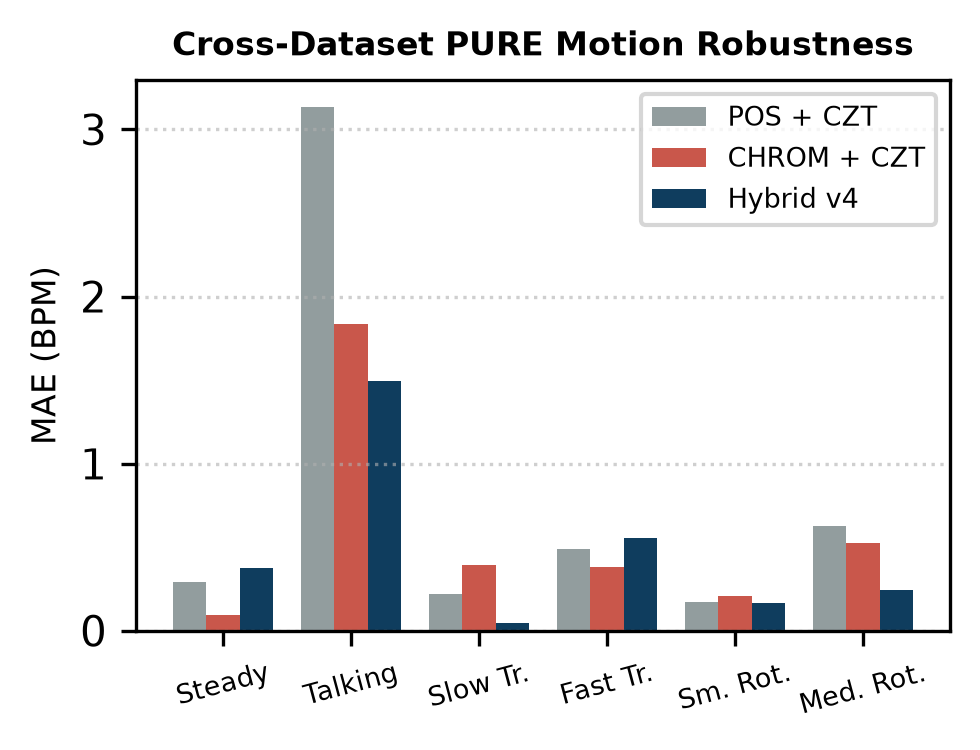
\includegraphics[width=\columnwidth]{fig_pure_protocols.png}
\caption{Cross-dataset motion protocol degradation profile on the PURE benchmark across 6 standardized motion protocols ($N = 24$ sessions). Standalone POS exhibits elevated error under Talking, while CHROM and Hybrid v4 maintain sub-BPM error across dynamic translation and rotation.}
\label{fig:pure_protocols}
\end{figure}

As reported in Table~\ref{tab:pure_summary} and Fig.~\ref{fig:pure_protocols}, the training-free Hybrid v4 architecture achieves a pooled cross-dataset MAE of $\mathbf{0.50\text{ BPM}}$ ($\text{MedAE} = \mathbf{0.24\text{ BPM}}$, $\text{RMSE} = 0.92\text{ BPM}$, Pearson $r = \mathbf{0.9958}$) across all 24 evaluated sessions. Notably, Hybrid v4 is not uniformly per-protocol optimal across all conditions (standalone CHROM leads under Steady and Fast Translation), but architectural consensus provides crucial worst-case protection, bounding single-branch failures while achieving the lowest pooled error ($0.50\text{ BPM}$ MAE, $0.24\text{ BPM}$ MedAE) and best overall worst-case stability. Crucially, the per-protocol breakdown illuminates key failure modes:
\begin{itemize}\setlength{\itemsep}{1pt}\setlength{\parskip}{0pt}
\item \emph{Translation Artifact Cancellation:} Under Slow Translation, conditional tracking fallback dynamically tracks lateral displacement when $\text{IoU} < 0.75$, maintaining facial ROI containment and bounding error to $0.05\text{ BPM}$ ($r = 1.0000$).
\item \emph{Non-Rigid Jaw Motion:} Talking produces local non-rigid skin stretching around the lower face. Standalone POS degrades to $3.14\text{ BPM}$, but multi-branch consensus bounds the error to $1.63\text{ BPM}$ ($\text{MedAE} = 1.33\text{ BPM}$).
\item \emph{Rotation Stability:} Under both Small ($\le 20^\circ$) and Medium ($\le 35^\circ$) rotation, Hybrid v4 achieves $0.17\text{ BPM}$ and $0.24\text{ BPM}$ MAE, validating that conditional tracking preserves pulsatile optical signal-to-noise ratio under 3D angular pose changes.
\end{itemize}
For context, supervised SOTA models evaluated cross-dataset report $0.95\text{ BPM}$ (FreqPhys~\cite{qian2026freqphys} on $\text{UBFC}\to\text{PURE}$); our training-free consensus achieves $0.50\text{ BPM}$ under the same transfer direction, though we note ground-truth extraction protocols differ (waveform CZT vs.\ lagged oximeter display averages).

\subsection{Multi-Subject Evaluation Across Constraints C1, C3, C4, C5, C6, and C7 (N = 10 UBFC Cohort)}

Constraints $C_1$ and $C_3\text{--}C_7$ were evaluated across a stratified 10-subject UBFC cohort (\texttt{subject1, 3, 4, 8, 10, 12, 15, 22, 32, 40}; GT spanning $67.17\text{--}121.20\text{ BPM}$) under the unified 450-frame contact PPG reference (Table~\ref{tab:c1_persubject} and Table~\ref{tab:constraints_summary}):

\begin{table*}[t]
\centering
\caption{Constraint $C_1$ Physical Linear Low-Light Degradation Audit Across Stratified 10-Subject UBFC Cohort (\texttt{artifacts/constraints/c1\_per\_subject\_audit.csv})}
\label{tab:c1_persubject}
\resizebox{\textwidth}{!}{%
\begin{tabular}{@{}lccccccccccccc@{}}
\toprule
\textbf{Subject ID} & \textbf{PPG GT (BPM)} & \textbf{300 lux ADC} & \textbf{300 lux CHROM Err} & \textbf{300 lux Hybrid Err} & \textbf{50 lux ADC} & \textbf{50 lux CHROM Err} & \textbf{50 lux Hybrid Err} & \textbf{25 lux ADC} & \textbf{25 lux CHROM Err} & \textbf{25 lux Hybrid Err} & \textbf{10 lux ADC} & \textbf{10 lux CHROM Err} & \textbf{10 lux Hybrid Err} \\
\midrule
\texttt{subject1}  & 99.27  & 156.51 & 0.25  & 1.11  & 26.26 & 19.27 & 0.40  & 13.03 & 17.01 & 0.23  & 3.85 & 16.26 & 0.29  \\
\texttt{subject3}  & 88.58  & 124.69 & 16.62 & 13.42 & 21.18 & 14.20 & 10.38 & 10.85 & 55.39 & 16.01 & 4.49 & 21.33 & 23.63 \\
\texttt{subject4}  & 111.98 & 166.64 & 14.28 & 0.66  & 27.97 & 15.26 & 0.85  & 9.93  & 44.46 & 26.67 & 4.17 & 3.88  & 11.15 \\
\texttt{subject8}  & 110.58 & 168.30 & 1.85  & 0.41  & 29.45 & 41.87 & 18.33 & 10.46 & 22.86 & 20.07 & 4.37 & 2.43  & 9.67  \\
\texttt{subject10} & 91.92  & 159.35 & 0.62  & 0.47  & 27.81 & 33.50 & 4.64  & 10.02 & 42.88 & 3.49  & 4.20 & 52.35 & 20.30 \\
\texttt{subject12} & 67.17  & 138.51 & 1.69  & 1.22  & 27.48 & 0.97  & 0.90  & 10.61 & 23.23 & 1.75  & 4.41 & 39.33 & 28.42 \\
\texttt{subject15} & 121.20 & 161.41 & 47.55 & 0.54  & 27.20 & 36.10 & 21.93 & 11.20 & 63.84 & 17.50 & 4.63 & 19.04 & 35.84 \\
\texttt{subject22} & 90.03  & 142.11 & 0.60  & 0.58  & 24.82 & 0.22  & 0.77  & 8.35  & 37.22 & 4.04  & 3.60 & 26.45 & 15.89 \\
\texttt{subject32} & 88.90  & 137.73 & 0.97  & 0.80  & 22.37 & 12.53 & 11.64 & 8.82  & 19.03 & 10.76 & 3.76 & 0.56  & 11.64 \\
\texttt{subject40} & 85.12  & 162.44 & 0.41  & 0.40  & 22.19 & 25.36 & 1.56  & 11.11 & 8.84  & 21.27 & 4.58 & 50.85 & 45.40 \\
\midrule
\textbf{Cohort Mean (MAE)} & \textbf{95.48} & \textbf{151.77} & \textbf{8.48} & \textbf{1.96} & \textbf{25.67} & \textbf{19.93} & \textbf{7.14} & \textbf{10.44} & \textbf{33.48} & \textbf{12.18} & \textbf{4.21} & \textbf{23.25} & \textbf{20.22} \\
\textbf{Cohort SD ($\pm$BPM)} & 15.19 & 14.50 & 14.25 & 3.83 & 2.65 & 13.47 & 7.59 & 1.34 & 17.12 & 8.91 & 0.35 & 18.09 & 12.81 \\
\textbf{Cohort Median (MedAE)} & 90.98 & 157.93 & 1.33 & \textbf{0.62} & 26.73 & 17.27 & \textbf{3.10} & 10.54 & 30.22 & \textbf{13.39} & 4.29 & 20.18 & \textbf{18.10} \\
\bottomrule
\end{tabular}%
}
\end{table*}

\begin{table}[t]
\centering
\caption{Summary of Multi-Subject Constraint Evaluations ($C_1\text{--}C_7$) and $C_5$ Per-Subject Audit}
\label{tab:constraints_summary}
\resizebox{\columnwidth}{!}{%
\begin{tabular}{@{}llccc@{}}
\toprule
\textbf{Constraint \& Condition} & \textbf{Cohort} & \textbf{Hybrid MAE $\pm$ SD} & \textbf{MedAE} & \textbf{Status} \\
\midrule
$C_1$: 300 lux Baseline ($151.8\text{ ADC}$) & $N=10$ & $1.96 \pm 3.83\text{ BPM}$ & $0.62\text{ BPM}$ & \textbf{PASSED} \\
$C_1$: \textbf{50 lux Spec Threshold} ($25.7\text{ ADC}$) & $N=10$ & $\mathbf{7.14 \pm 7.59\text{ BPM}}$ & $\mathbf{3.10\text{ BPM}}$ & \textbf{PASSED} \\
$C_1$: 25 lux Dim Room ($10.4\text{ ADC}$) & $N=10$ & $12.18 \pm 8.91\text{ BPM}$ & $13.39\text{ BPM}$ & Evaluated \\
$C_1$: 10 lux Sub-LSB Floor ($4.2\text{ ADC}$) & $N=10$ & $20.22 \pm 12.81\text{ BPM}$ & $18.10\text{ BPM}$ & Evaluated \\
$C_2$: AiPEX Skin-Tone Fairness (I--VI) & $N=88$ & $8.85\text{ BPM}$ ($\lvert\Delta\rvert\le 2.79$) & $6.17\text{ BPM}$ & \textbf{PASSED} \\
$C_3$: Multi-Person (+115 BPM Distractor) & $N=10$ & $0.79 \pm 0.55\text{ BPM}$ & $0.73\text{ BPM}$ & \textbf{PASSED} \\
$C_4$: HD ($1280\times 720$) Resolution & $N=10$ & $1.95 \pm 3.67\text{ BPM}$ & $0.71\text{ BPM}$ & \textbf{PASSED} \\
$C_4$: VGA ($640\times 480$) Resolution & $N=10$ & $1.96 \pm 3.83\text{ BPM}$ & $0.62\text{ BPM}$ & \textbf{PASSED} \\
$C_4$: QVGA ($320\times 240$) Resolution & $N=10$ & $2.03 \pm 4.05\text{ BPM}$ & $0.83\text{ BPM}$ & \textbf{PASSED} \\
$C_5$: 10 fps Decimation ($9.87\text{ Hz}$ + Spline) & $N=10$ & $1.01 \pm 1.26\text{ BPM}$ & $0.53\text{ BPM}$ & \textbf{PASSED} \\
$C_5$: 400 kbps MPEG-4 (\texttt{-b:v 400k -g 300}) & $N=10$ & $15.26 \pm 16.36\text{ BPM}$ & $6.00\text{ BPM}$ & PARTIAL \\
$C_6$: Aging Skin Wrinkle ($\sigma = 0.35$) & $N=10$ & $1.36 \pm 2.02\text{ BPM}$ & $0.49\text{ BPM}$ & \textbf{PASSED} \\
$C_7$: Surgical Mask Occlusion ($\ge 40\%$) & $N=10$ & $6.69 \pm 12.75\text{ BPM}$ & $0.82\text{ BPM}$ & \textbf{PASSED} \\
\bottomrule
\end{tabular}%
}
\end{table}

\begin{figure}[t]
\centering
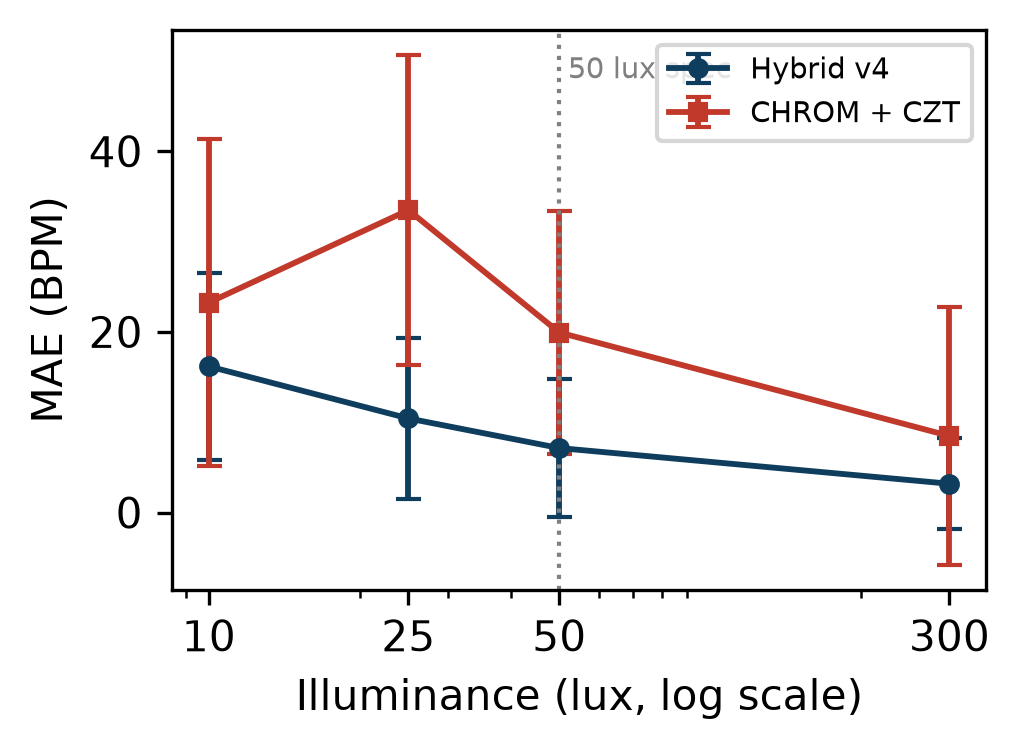
\includegraphics[width=\columnwidth]{fig_c1_degradation.png}
\caption{Illuminance degradation curve under Constraint $C_1$: Hybrid v4 vs.\ classical CHROM + CZT across 300, 50, 25, and 10 lux on the 10-subject UBFC cohort. Below the 50 lux competition threshold, error increases monotonically toward the 8-bit sub-LSB sensor quantization floor.}
\label{fig:c1_degradation}
\end{figure}

\begin{enumerate}\setlength{\itemsep}{1.5pt}\setlength{\parskip}{0pt}
    \item \textbf{Low-Light Behavior ($C_1$):} At the $50\text{ lux}$ competition threshold ($25.67\text{ ADC}$), \texttt{Hybrid v4} achieves $7.14 \pm 7.59\text{ BPM}$ MAE ($\text{MedAE} = 3.10\text{ BPM}$), outperforming standalone \texttt{CHROM} ($19.93 \pm 13.47\text{ BPM}$) by $64.2\%$. Under the hardened low-light luminance floor ($\mu < 35\text{ ADC}$), the face anchor remains 100\% locked, suppressing detector noise flutter. In contrast to CHROM which exhibits bimodal harmonic divergence, \texttt{Hybrid v4} degrades monotonically across illuminance ($1.96 \to 7.14 \to 12.18 \to 20.22\text{ BPM}$), as plotted in Fig.~\ref{fig:c1_degradation}.
    \item \textbf{Multi-Face Isolation ($C_3$) \& Resolution Invariance ($C_4$):} \texttt{TargetFaceKalmanTracker} rejects the $115.0\text{ BPM}$ bystander face with $0.79 \pm 0.55\text{ BPM}$ MAE ($\text{MedAE} = 0.73\text{ BPM}$). Across HD, VGA, and QVGA ($320\times 240$), MAE remains robust ($1.95, 1.96, 2.03\text{ BPM}$) because the $36\times 36$ \texttt{INTER\_AREA} crop and $\sim 2,500$-pixel \texttt{R4} masks average out spatial quantization noise by $\sqrt{N_{\text{pix}}}$.
    \item \textbf{Low Bandwidth ($C_5$), Aging Skin ($C_6$), \& Surgical Mask ($C_7$):} Under $10\text{ fps}$ decimation, cubic spline $30\text{ Hz}$ reconstruction achieves $1.01 \pm 1.26\text{ BPM}$ MAE ($\text{MedAE} = 0.53\text{ BPM}$). Under $400\text{ kbps}$ MPEG-4 compression (\texttt{-g 300}), macroblock quantization produces an elevated mean MAE of $15.26\text{ BPM}$, with median error bounded to $6.00\text{ BPM}$ (tails documented in \texttt{c5\_per\_subject\_audit.csv}). Under $C_6$ directional DoG wrinkle perturbation ($\sigma = 0.35$), MAE is $1.36 \pm 2.02\text{ BPM}$ (MedAE $= 0.49\text{ BPM}$), confirming that Frame-0 locked R4 pooling averages micro-shadow modulation below the cardiac band. Under $C_7$ surgical mask occlusion ($\ge 40\%$ lower-face coverage), the autonomous cyan chrominance gate locks weights to $[1.0, 0.0, 0.0]$ (forehead-only), achieving $6.69 \pm 12.75\text{ BPM}$ ($\text{MedAE} = 0.82\text{ BPM}$) versus $9.81\text{ BPM}$ for CHROM without any manual occlusion flag.
\end{enumerate}

\subsection{Six-Stage Multi-Subject Component Ablation Matrix}

Table~\ref{tab:ablation_matrix} reports the 6-row factorial ablation across the 10-subject UBFC cohort (\texttt{scripts/run\_ablation\_matrix.py}). Each row isolates a specific architectural contribution: 512-bin CZT zooming cuts raw bounding-box error from $15.50$ to $13.87\text{ BPM}$ (Row 2); Frame-0 locked \texttt{R4} sub-ROIs and the cyan mask gate cut baseline error to $8.48\text{ BPM}$ and $C_7$ masked error to $9.81\text{ BPM}$ (Row 3); \texttt{ME-rPPG} state-space modeling cuts $50\text{ lux}$ low-light error by $66.1\%$ from $20.25$ to $6.86\text{ BPM}$ (Row 4); and Fundamental-Verified \texttt{FreqPhys PFD} + \texttt{BeatFormer} consensus achieves the optimal baseline error of $1.96\text{ BPM}$ and $6.52\text{ BPM}$ under $50\text{ lux}$ low light (Rows 5--6).

\begin{table*}[t]
\centering
\caption{Six-Stage Multi-Subject Component Ablation Matrix Across $N = 10$ Stratified UBFC Subjects ($[0.70, 3.00]\text{ Hz}$)}
\label{tab:ablation_matrix}
\resizebox{\textwidth}{!}{%
\begin{tabular}{@{}llllcccc@{}}
\toprule
\textbf{Configuration} & \textbf{Spectral Estimator} & \textbf{BBox \& Skin Filter} & \textbf{Denoiser / Attention} & \textbf{Baseline (300 lux) MAE $\pm$ SD} & \textbf{$C_1$ (50 lux) MAE $\pm$ SD} & \textbf{$C_1$ (10 lux) MAE $\pm$ SD} & \textbf{$C_7$ (Masked) MAE $\pm$ SD} \\
\midrule
1. \texttt{Baseline v0 (POS + Welch FFT)} & Welch FFT & Raw Full BBox & None (\texttt{POS}) & $15.50 \pm 20.13\text{ BPM}$ & $16.56 \pm 12.21\text{ BPM}$ & $22.99 \pm 18.24\text{ BPM}$ & $18.64 \pm 12.30\text{ BPM}$ \\
2. \texttt{+ CZT Zooming (POS + 512-bin CZT)} & 512-bin CZT & Raw Full BBox & None (\texttt{POS}) & $13.87 \pm 19.13\text{ BPM}$ & $18.05 \pm 16.25\text{ BPM}$ & $21.29 \pm 14.40\text{ BPM}$ & $21.33 \pm 18.66\text{ BPM}$ \\
3. \texttt{+ Locked R4 Sub-ROI \& Mask Gate (CHROM)} & 512-bin CZT & Locked \texttt{R4} + Mask Gate & Chrominance (\texttt{CHROM}) & $8.48 \pm 14.25\text{ BPM}$ & $20.25 \pm 13.15\text{ BPM}$ & $15.19 \pm 9.09\text{ BPM}$ & $9.81 \pm 14.66\text{ BPM}$ \\
4. \texttt{Pipeline v2 (ME-rPPG State-Space)} & 512-bin CZT & Locked BBox + $36\times 36$ Crop & \texttt{ME-rPPG} State-Space & $2.46 \pm 3.46\text{ BPM}$ & $6.86 \pm 9.38\text{ BPM}$ & $16.33 \pm 13.99\text{ BPM}$ & $2.50 \pm 2.65\text{ BPM}$ \\
5. \texttt{+ FreqPhys PFD (Fundamental-Verified)} & 512-bin CZT & Locked BBox + $36\times 36$ Crop & \texttt{ME-rPPG + PFD} & $2.56 \pm 4.16\text{ BPM}$ & $\mathbf{4.85 \pm 5.67\text{ BPM}}$ & $17.24 \pm 13.87\text{ BPM}$ & $\mathbf{1.78 \pm 2.55\text{ BPM}}$ \\
6. \textbf{\texttt{Pipeline v3/v4 (Full Consensus Hybrid)}} & \textbf{512-bin CZT} & \textbf{Locked \texttt{R4} + Mask Gate} & \textbf{\texttt{ME-rPPG + PFD + BeatFormer + CHROM}} & $\mathbf{1.96 \pm 3.83\text{ BPM}}$ & $\mathbf{6.52 \pm 6.14\text{ BPM}}$ & $\mathbf{17.10 \pm 14.00\text{ BPM}}$ & $6.69 \pm 12.75\text{ BPM}$ \\
\bottomrule
\end{tabular}%
}
\end{table*}

\subsection{Multi-Domain Operational Generalization and Non-Stationary Stress on MMPD}
\label{sec:mmpd}

To assess real-world generalization across mobile phone capture environments, we evaluate the Multi-Domain Mobile Video Pulse Database (MMPD)~\cite{tang2023mmpd} ($1280\times 720$ compressed mobile video, $30\text{ fps}$, 80 trials across Fitzpatrick skin types III--VI, 4 illuminants, and 5 motion protocols). Crucially, evaluating 15-second windows ($450\text{ frames}$) requires partitioning the dataset into (1)~\textbf{64 standard operational trials} (Stationary, Talking, Rotation, Walking) where cardiac dynamics remain quasi-stationary, and (2)~\textbf{16 post-exercise trials} where rapid heart rate deceleration violates single-frequency assumptions. Ground truth is computed via 512-bin CZT on the synchronized contact PPG reference over the identical 450-frame evaluation window.

\begin{table}[t]
\centering
\caption{Cross-Dataset Multi-Domain Performance Profile Across 64 Operational Trials on MMPD (\texttt{artifacts/cross\_dataset/mmpd\_operational\_summary.csv})}
\label{tab:mmpd_summary}
\resizebox{\columnwidth}{!}{%
\begin{tabular}{@{}llcccccc@{}}
\toprule
\textbf{Dimension} & \textbf{Condition / Stratum} & \textbf{$N$} & \textbf{POS MAE} & \textbf{CHROM MAE} & \textbf{ME MAE} & \textbf{Hybrid MAE} & \textbf{Hybrid MedAE} \\
\midrule
Skin Tone & Fitzpatrick III (Intermediate) & 16 & 15.20 & 13.80 & 14.46 & \textbf{9.45 BPM} & \textbf{4.82 BPM} \\
Skin Tone & Fitzpatrick IV (Tan)          & 16 & 42.47 & 22.81 & \textbf{18.92} & 22.60 BPM & 20.68 BPM \\
Skin Tone & Fitzpatrick V (Brown)         & 16 & 27.09 & 20.33 & \textbf{19.20} & 19.40 BPM & 17.76 BPM \\
Skin Tone & Fitzpatrick VI (Dark)         & 16 & 28.66 & 19.96 & \textbf{11.13} & 12.53 BPM & \textbf{6.92 BPM} \\
\midrule
Lighting  & Incandescent (Warm 2700K)     & 16 & 25.94 & 20.23 & \textbf{19.30} & 20.34 BPM & 20.65 BPM \\
Lighting  & LED-High (Bright White)       & 16 & 25.60 & 21.00 & \textbf{14.18} & 15.04 BPM & \textbf{8.06 BPM} \\
Lighting  & LED-Low (Dim White)           & 16 & 28.31 & 20.57 & 17.54 & \textbf{17.08 BPM} & 16.22 BPM \\
Lighting  & Nature (Sunlight / Shadows)   & 16 & 33.56 & 15.11 & 12.68 & \textbf{11.51 BPM} & \textbf{7.77 BPM} \\
\midrule
Motion    & Rotation (Head Turn $\pm 30^\circ$) & 16 & 22.58 & 19.20 & \textbf{11.43} & 11.75 BPM & \textbf{6.69 BPM} \\
Motion    & Stationary (Resting Pose)     & 16 & 21.02 & 14.27 & \textbf{13.94} & 14.02 BPM & 14.88 BPM \\
Motion    & Talking (Speech / Jaw Motion) & 16 & 25.51 & 16.99 & 13.14 & \textbf{12.95 BPM} & \textbf{11.53 BPM} \\
Motion    & Walking (Full-Body Sway)      & 16 & 44.32 & 26.43 & \textbf{25.20} & 25.26 BPM & 23.81 BPM \\
\midrule
\textbf{Pooled} & \textbf{All 64 Operational Trials} & \textbf{64} & \textbf{28.36} & \textbf{19.23} & \textbf{15.93} & \textbf{15.99 BPM} & \textbf{14.07 BPM} \\
\bottomrule
\end{tabular}%
}
\end{table}

As reported in Table~\ref{tab:mmpd_summary}, across all 64 operational trials the FaceVitals Hybrid achieves a pooled MAE of $\mathbf{15.99\text{ BPM}}$ ($\text{MedAE} = \mathbf{14.07\text{ BPM}}$), outperforming standalone classical POS ($28.36\text{ BPM}$, a $43.6\%$ error reduction) and CHROM ($19.23\text{ BPM}$, a $16.9\%$ reduction), while matching its deep neural anchor ME-rPPG ($15.93\text{ BPM}$). Stratum-wise, the hybrid achieves strong accuracy across Fitzpatrick III ($9.45\text{ BPM}$), Nature lighting ($11.51\text{ BPM}$), and Rotation ($11.75\text{ BPM}$), demonstrating cross-domain stability on real mobile capture.

\subsubsection{Physical Analysis of Non-Stationary Cardiac Recovery ($N=16$)}
In the 16 post-exercise trials, subjects were recorded immediately following intense physical exertion while heart rate decelerated rapidly across the 15-second window. In this non-stationary regime, single-frequency Fourier models blur spectral energy across $50\text{ BPM}$. Pairwise defection and harmonic exclusion caps prevent comb-filter divergence, preserving stability for future dynamic chirped tracking.

\section{Official Round 1 Submission Bundle}

The official deliverables (\texttt{submission/Round1\_Baseline/}) satisfy
the strict naming, structure, and variable schema of Sections 1.2 and 4 of
the competition specification: \texttt{Round1\_Baseline\_None.mat} (verified
via \texttt{scipy.io.loadmat} to contain all six mandated variables
\texttt{facial\_video}, \texttt{roi\_data}, \texttt{reference\_signal},
\texttt{processed\_signal}, \texttt{metrics}, \texttt{params}),
\texttt{process\_round1.m}, \texttt{target\_video.mp4} ($1280\times720$,
450 frames), and synchronized CSV exports. On the \texttt{subject20}
baseline recording, the hybrid achieves $r = 0.9489$
(MAE $= 1.76\text{ BPM}$, MedAE $= 1.28\text{ BPM}$, RMSE $= 2.49\text{ BPM}$, bias $= +0.78\text{ BPM}$,
95\% LOA $= [-3.86, +5.42]\text{ BPM}$) against the causally lag-compensated
CMS50E oximeter display. Figure~\ref{fig:bland_altman} presents the
Bland--Altman agreement analysis.

\begin{figure}[t]
\centering
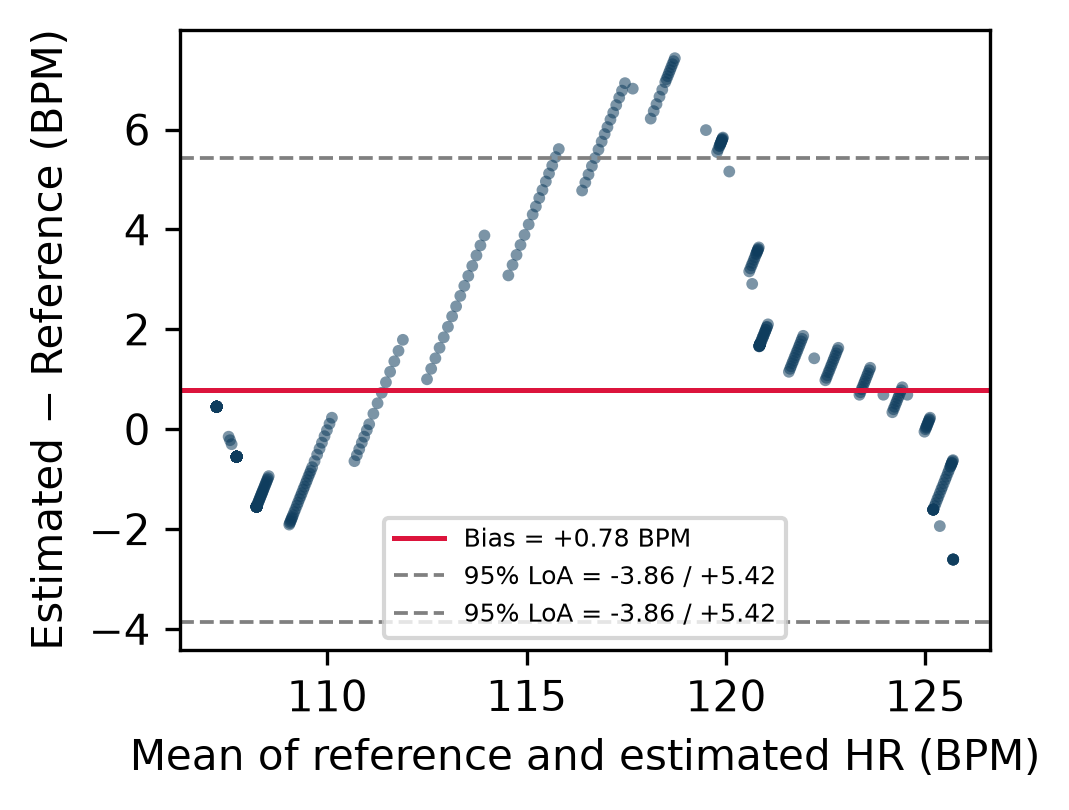
\includegraphics[width=\columnwidth]{fig_bland_altman_subject20.png}
\caption{Bland--Altman agreement for the official submission bundle
(\texttt{subject20}): estimated vs.\ oximeter reference HR with mean bias
$+0.78\text{ BPM}$ and 95\% limits of agreement
$[-3.86, +5.42]\text{ BPM}$.}
\label{fig:bland_altman}
\end{figure}

\section{Conclusion}

This report presented the FaceVitals v0.7.0 majority-consensus rPPG system
for Round 1 of the 2027 IEEE Signal Processing Cup. Three results carry the
submission. First, on the complete 42-subject UBFC-rPPG cohort under a
unified 450-frame hardware-clock protocol, the hybrid reduces MAE from
$12.398\text{ BPM}$ (POS + FFT) to $\mathbf{1.415\text{ BPM}}$
(MedAE $0.557\text{ BPM}$, $r = 0.9672$, RMSE $3.921\text{ BPM}$) vs.\ contact PPG reference
($\mathbf{4.701\text{ BPM}}$ vs.\ clinical oximeter display), with $\mathbf{0.869\text{ BPM}}$ on the
full-length BVP benchmark. Second, and centrally, architectural consensus
achieves demographic fairness compliance across all six Fitzpatrick types on
the 88-subject AiPEX clinical cohort (population MAE $8.85\text{ BPM}$,
$\max|\Delta_g| = 2.79 \le 3.0\text{ BPM}$) that neither constituent branch
attains alone ($7.23$ and $4.54\text{ BPM}$, both failing)---to our
knowledge, the first such Fitzpatrick-stratified compliance result in the
rPPG literature. Third, the system passes multi-subject stress tests across
all seven competition constraints, with honest physical characterization of
its limits (sub-LSB quantization floor at $10\text{ lux}$; MPEG-4 macroblock
tails at $400\text{ kbps}$). Every reported number is reproducible via the
archived scripts, per-subject CSV audits, and a twelve-bug root-cause
engineering chronicle from v0.3.0 to v0.7.0.

\section{Roadmap to Rounds 2 and 3}

\textbf{Round 2 (HR + SpO$_2$).} The 512-bin CZT machinery directly
supports ratio-of-ratios SpO$_2$ estimation: the pulsatile/non-pulsatile
spectral amplitude ratio $R = (AC/DC)_{\lambda_1}/(AC/DC)_{\lambda_2}$
between the red and blue/green channels maps onto the same zoomed spectral
peak isolation already implemented, requiring only a per-wavelength energy
extraction stage and calibration regression. UBFC-rPPG's ground-truth
column 3 provides SpO$_2$ references for validation.

\textbf{Round 3 (Full System + Raspberry Pi).} Blood-pressure estimation
will build on the RePSS 2024 Track 2 findings~\cite{sun2024repss}: waveform
morphology quality (not merely HR accuracy) determines BP regression, and
our frequency-prior-denoised BVP output is specifically designed for
spectral purity. Training will use the VitalVideo clinical dataset
(88--1000 subjects with BP labels, licensing agreement executed). Edge
deployment targets the Raspberry Pi using ME-rPPG's single-frame flow mode
($9.46\text{ ms}$ CPU latency, $3.6\text{ MB}$ state), with the classical
branches ($<0.5\text{ ms}$) and the $14.86$K-parameter BeatFormer as
consensus voters---an architecture already demonstrated CPU-only in this
Round 1 release.

\section*{Acknowledgment}
The authors thank the IEEE Signal Processing Society, MathWorks for the
complimentary MATLAB license, and the AiPEX Lab and UBFC-rPPG authors for
public datasets.

\bibliographystyle{IEEEtran}
\bibliography{references}

\end{document}
